% --------------------------------------------------------------------------------
% Student guideline for the final year dissertation using LaTeX2e
% Alexandra Bonnici
% Department of Systems and Control
% 13th September 2017

\documentclass[12pt, oneside]{Thesis}

% --------------------------------------------------------------------------------
% Some useful packages
% You may add/remove any packages as you deem fit,
% Recommended packages which are recommended are marked by [R] in the comment
% --------------------------------------------------------------------------------

% font options & general typesetting
\usepackage{microtype}            % some refinements over the general appearance of text
\usepackage{eqparbox}             % ensures that blocks of text occupy the same space

% for figures
\usepackage[]{graphicx}     %  [R] to use graphics
\usepackage{subfigure}            %  [R] to make subfigures
\usepackage{epstopdf}             %  [R] adds eps support in the graphics package
\usepackage{wrapfig}              %  to allow text to wrap around figures


% for tables
\usepackage[table]{xcolor}
\usepackage{multirow,bigstrut}    % to have tables with merged rows
\usepackage{array, booktabs}      %  [R] for good looking tables
\usepackage{longtable}            % to create tables that span more than one page
\usepackage{adjustbox}            % so that long tables fit within the page
\usepackage{rotating}             % adds support to rotate pages

% to write nice mathematical equations
\usepackage{mathtools}            %  [R] some mathematical tools
\usepackage{amsmath}		      %  [R] to write math formulas easily
\usepackage{amssymb}              %  [R] for maths symbols
\usepackage{amsthm}               % for the typesetting of theorems
\usepackage{esvect}               % to make vector arrows
\usepackage{bm}                   % to make bold maths symbols

\usepackage{xfrac}                % [R] to make in-text fractions

% more symbols
\usepackage{pifont}               % Postscript standard Symbol and Dingbats fonts
\usepackage{gensymb}              % generic symbols fonts
\usepackage{stackrel}             % to stack things on top of each other

% to include urls
\usepackage{url}                  % to write urls

% to typeset pseudo code algorithms and source codes
\usepackage{algorithm}            % to type set algorithms as pseudo code
\usepackage{algpseudocode}        % more layout options for algorithm pseudo code
\usepackage{listings}             % to add non-formatted text e.g. source code

\usepackage{tabularx}
\usepackage{multirow}
\usepackage{todonotes}
\usepackage{adjustbox}

\definecolor{mGreen}{rgb}{0,0.6,0}
\definecolor{mGray}{rgb}{0.5,0.5,0.5}
\definecolor{mPurple}{rgb}{0.58,0,0.82}
\definecolor{backgroundColour}{rgb}{0.95,0.95,0.92}

\lstdefinestyle{LuaStyle}
{
  backgroundcolor   = \color{backgroundColour},
  commentstyle      = \color{mGreen},
  keywordstyle      = \color{magenta},
  numberstyle       = \tiny\color{mGray},
  stringstyle       = \color{mPurple},
  basicstyle        = \footnotesize,
  % breakatwhitespace = false,
  % breaklines        = true,
  captionpos        = b,
  keepspaces        = true,
  numbers           = left,
  numbersep         = 5pt,
  showspaces        = false,
  showstringspaces  = false,
  showtabs          = false,
  tabsize           = 2,
  language          = {[5.2]Lua},
}
\lstset{style=LuaStyle}

\lstdefinestyle{CStyle}{
    backgroundcolor   = \color{backgroundColour},
    commentstyle      = \color{mGreen},
    keywordstyle      = \color{magenta},
    numberstyle       = \tiny\color{mGray},
    stringstyle       = \color{mPurple},
    basicstyle        = \footnotesize,
    % breakatwhitespace = false,
    % breaklines        = true,
    captionpos        = b,
    keepspaces        = true,
    numbers           = left,
    numbersep         = 5pt,
    showspaces        = false,
    showstringspaces  = false,
    showtabs          = false,
    tabsize           = 2,
    language          = C,
}
% to typeset theorems, lemmas and definitions
\newtheorem{theorem}{Theorem}[chapter]
\newtheorem{lemma}{Lemma}
\newtheorem{definition}{Definition}

\newcommand{\paratitle}[1]{\underline{\textbf{\emph{#1}}}}
\newcommand{\keyword}[1]{\textcolor{red}{\emph{#1}}}
\lstnewenvironment{code}[1]
  {\noindent\lstset{style=#1Style}\adjustbox{bgcolor=backgroundColour,max width=\textwidth}\bgroup}
  {\egroup}

% --------------------------------------------------------------------------------
% Information relevant to your dissertation.
% Substitute with your own name, supervisor and title details.
%--------------------------------------------------------------------------------

\thesistitle{MAD-NG Performance Improvement} % title
\authors{
  Aurelien \textsc{Bloch}\\[1.5cm]
  Supervisor: Laurent \textsc{Deniau}\\
  EPFL supervisor: Martin \textsc{Odersky}
}
\keywords{LuaJIT, technical documentation}         	% keywords
%\department{}                						% department name
%\Udegree{}
\subject{LuaJIT Internals}
%\UNIVERSITY{}
%\faculty{Faculty of Engineering}

%\newif\ifHaveACosupervisor
% toggle the comment on the true/false lines as appropriate
%\HaveACosupervisortrue
%\HaveACosupervisorfalse

%--------------------------------------------------------------------------------
% Creates the PDF meta-data (for the electronic version of your dissertation).
% There is no need to modify this information
%--------------------------------------------------------------------------------
\hypersetup{urlcolor=blue,%
		        linkcolor=blue,%
            citecolor=blue,%
            colorlinks=true,%
            hypertexnames=true}

\hypersetup{pdftitle={\ttitle}}
\hypersetup{pdfsubject=\subjectname}
\hypersetup{pdfauthor=\authornames}
\hypersetup{pdfkeywords=\keywordnames}

%--------------------------------------------------------------------------------
% Creates the title page (typesetting is taken care of and details are as above)
%--------------------------------------------------------------------------------
\title{\ttitle}

%--------------------------------------------------------------------------------
% Creates the glossaries pages and index pages
%--------------------------------------------------------------------------------
\makeglossaries
\makeindex

%--------------------------------------------------------------------------------
% The actual start of the dissertation
%--------------------------------------------------------------------------------
\begin{document}

\frontmatter            % sets page numbers of the first few pages to roman
\setstretch{1.3}        % ensures a one-and-a-half line spacing
\fancyhead{}            % clears the headers
\rhead{\thepage}        % sets the top right header to the page number
\lhead{}                % ensures that the top left header remains empty
\pagestyle{fancy}     	% uses the "fancy" page style (adds the line at top)


%--------------------------------------------------------------------------------
% Prints out the title page
%--------------------------------------------------------------------------------
%!TEX root = ../FYP_Dissertation.tex
\begin{titlepage}

\begin{center}
\textsc{\large Computer Science\\ Master thesis\\ Spring 2018}
\end{center}

% \flushleft{\textsc{\large European Organization for Nuclear Research -- CERN}\\
% \large Beams Department --  Accelerators Beams Physics Group}

\vspace{2cm}
\begin{center}
\linespread{1.3}\huge \bfseries \ttitle
\end{center}
\vspace{2cm}
\begin{center}
by \\[1cm]
\authornames\\[6cm]

\includegraphics[height=2.5cm]{./Images/EPFL.eps}
\hspace{1cm}

\includegraphics[height=2.5cm]{./Images/CERN.eps}
\vfill
\end{center}

\end{titlepage}


% -------------------------------------------------------------------------------
% Prints out the copyright page (you do not need to modify this)
%--------------------------------------------------------------------------------
% \clearpage
% \Copyright{

\addtocontents{toc}{\vspace{1em}}
\vspace{2cm}

\begin{enumerate}
\item Copyright in text of this dissertation rests with the Author. Copies (by any process) either in full, or of extracts may be made only in accordance with regulations held by the Library of the University of Malta. Details may be obtained from the Librarian. This page must form part of any such copies made. Further copies (by any process) made in accordance with such instructions may not be made without the permission (in writing) of the Author.
\item Ownership of the right over any original intellectual property which may be contained in or derived from this dissertation is vested in the University of Malta and may not be made available for use by third parties without the written permission of the University, which will prescribe the terms and conditions of any such agreement.
\end{enumerate}}

%--------------------------------------------------------------------------------
% Prints out the abstract
% You will need to change the text in the file to reflect your own abstract
%--------------------------------------------------------------------------------
\clearpage
%!TEX root = ../FYP_Dissertation.tex
\addtotoc{Abstract}
\abstract{\addtocontents{toc}{\vspace{1em}}

TODO
}


%--------------------------------------------------------------------------------
% Prints out the acknowledgements page
% You will need to change the text to reflect your own acknowledgements
%--------------------------------------------------------------------------------
\clearpage
%!TEX root = ../FYP_Dissertation.tex
\setstretch{1.3}
\acknowledgements{\addtocontents{toc}{\vspace{1em}}
\vspace{2cm}
Firstly, I would like to express my sincere gratitude to my supervisor at CERN,
Laurent Deniau for the daily support during this entire project. I truly learned
a lot from this collaboration and opened my interested in new subjects.

Then, I would like to thank Prof. Martin Odersky to have accepted to be my EPFL
supervisor allowing me to pursue my work at CERN.

Finally, I would like to thank Mike Pall for his commitment to the LuaJIT project
from which I learned many things.

\vspace{1cm}
\emph{Meyrin, 27 August 2018} \hspace{5cm} \emph{Aurelien Bloch}
}




%--------------------------------------------------------------------------------
% Prints out the list of contents, figures and tables
% You don't have to modify any of this
%--------------------------------------------------------------------------------
\clearpage
\pagestyle{fancy}

\lhead{\emph{Contents}}
\tableofcontents

\lhead{\emph{List of Figures}}
\listoffigures

\lhead{\emph{List of Tables}}
\listoftables

%--------------------------------------------------------------------------------
% Prints out the list of acronyms
% No changes will be necessary if used properly within text
%--------------------------------------------------------------------------------
% \clearpage
% \setglossarystyle{altlist}
% \printglossary[type=\acronymtype, title=List of Acronyms, toctitle=List of Acronyms]

%--------------------------------------------------------------------------------
% Prints out the list of symbols
% No changes will be necessary if used properly within text, comment if not relevant
%--------------------------------------------------------------------------------

% \clearpage
% \setglossarystyle{list}
% \printglossary[title=List of Symbols,toctitle=List of Symbols]


%--------------------------------------------------------------------------------
% Prints out the chapter contents
%--------------------------------------------------------------------------------

\mainmatter
\pagestyle{fancy}

\part{Performance Analysis}
\label{Part:mad}

  \chapter{Introduction}
  \label{Chapt:Intro}

    \section{MAD}
    \label{Sec:mad}
    %!TEX root = ../../../FYP_Dissertation.tex

%===============================================================================
% Methodical Accelerator Design
%===============================================================================

\subsection{Methodical Accelerator Design}
\label{Subsec:mad-orig}

MAD or Methodical Accelerator Design is a complete set of tools bundle together
and developed at CERN to design, study, simulate and optimize beam physics for
particle accelerators. Its current version is called MAD-X. It was first released
in 2002 and is the successor of  MAD-8 (see official website \cite{madx}).
Its source code is mainly written in C, C++, Fortan77 and Fortran90.
It presents itself as a command-line program that reads and execute its custom
scripting language. This language has the particularity of having a single
workspace where everything is global. There is no function but a simple macro
system. Most of the functionalities are provided through high-level commands that
can be customized by the user. Deferred expressions are heavily used everywhere.
This code has been internally known to
be difficult to maintain and improve. In additions of that, developing new
functionality for it takes a significant amount of time due to the fact that
module are tightly coupled and modification on its big code base can have
unexpected side effect if the developer is not careful. The need for
consolidation plus the rise of efficient and modern languages making the
development faster and more flexible triggered a new redesign of the MAD
application called MAD-NG.


%===============================================================================
% MAD-NG
%===============================================================================

\subsection{MAD Next Generation}
\label{Subsec:mad-ng}

MAD-NG or Methodical Accelerator Design Next Generation is, like stated previously,
a modern redesign of the MAD application. The objectives of MAD-NG are, to use
a simple scripting language to offer easier and faster development, to propose
a well-compartmented and modular design for scalability, to allow much more
flexible user input, to reintroduce computer science good practices with scopes,
functions, control-flow, etc.. It has to do so while being at least as performant
as MAD-X, keeping the high level command-like philosophy and staying a standalone
single binary working out of the box without any installation procedure.
The scripting language Lua through LuaJIT as been picked (see Section \ref{Sec:LuaJIT}).\\


\subsubsection{MAD-NG packaging}
\label{Subsec:mad-pk}

Figure \ref{fig:mad} shows how the MAD-NG application is being packaged. Some
modification over LuaJIT has been done to allow it to be embedded inside of MAD.
The source code of MAD is mainly implemented in lua (\emph{*.mad} extension
files) but for performance reasons some physic calculations and algorithms are
written in \emph{C}. A big advantage of LuaJIT is the efficiency of the FFI
library (Foreign Function Interface) that allows to use embedded \emph{C} code
or even \emph{C} libraries directly inside the lua application.

\begin{figure}[H]
    \centering
	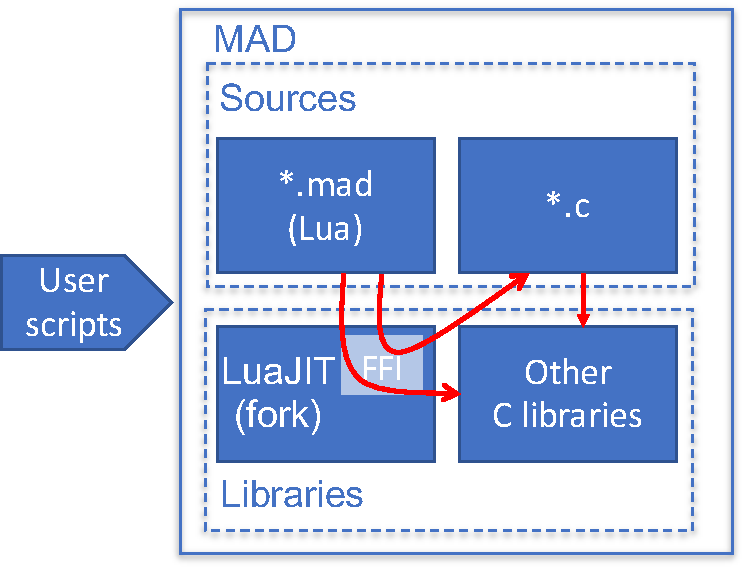
\includegraphics[width=7cm]{./Images/MAD.pdf}
    \caption{MAD-NG application}
    \label{fig:mad}
\end{figure}

\subsubsection{MAD-NG modules overview}
\label{Subsec:mad-doc}

This section does not attempt to provide a full documentation of MAD but a
minimum amount to be able to understand the rest of this dissertation.
Figure \ref{fig:mad-graph} below is a graph representing the different
modules currently available in MAD and the way they are connected.

\begin{figure}[H]
    \centering
	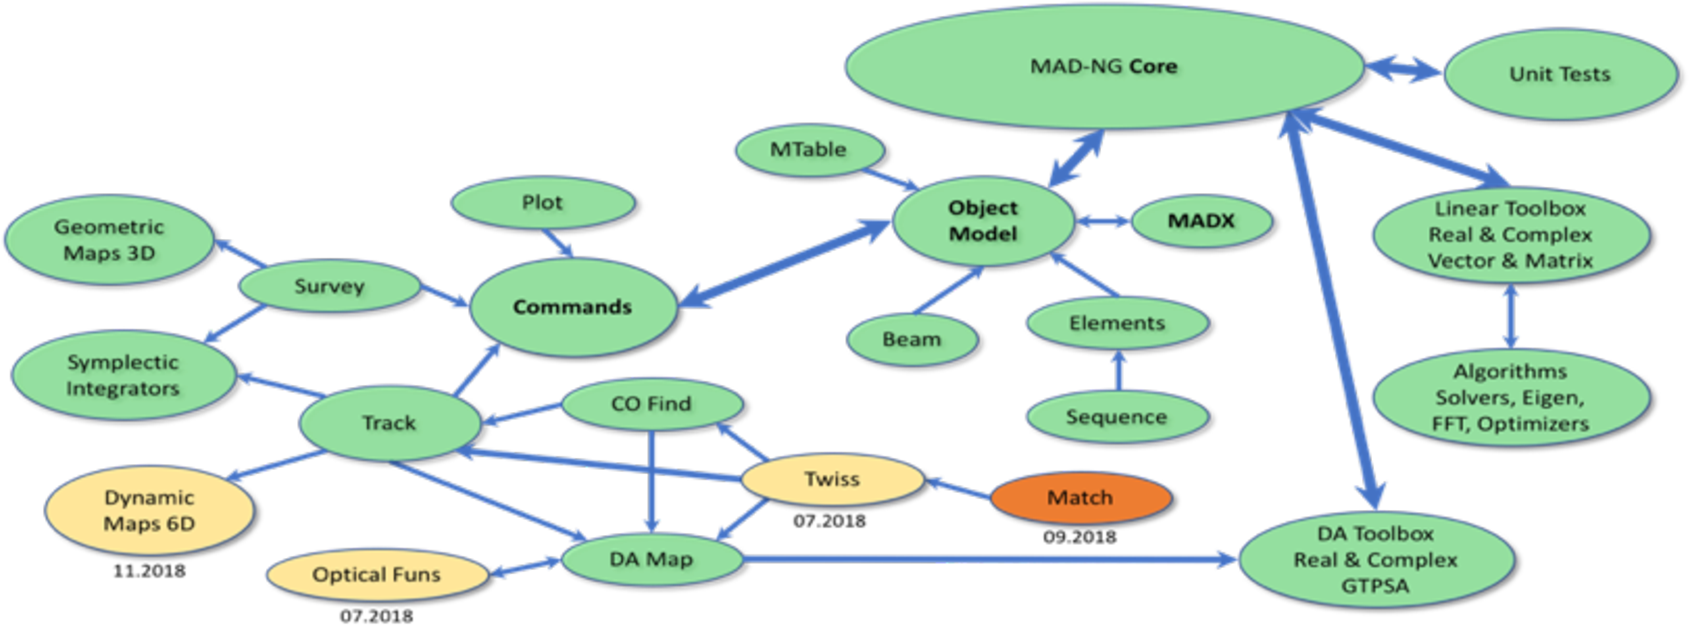
\includegraphics[width=\textwidth]{./Images/mad-graph.pdf}
    \caption{Current module hierarchy of MAD-NG}
    \label{fig:mad-graph}
\end{figure}

The two backbone modules are \emph{Object} and \emph{Commands}. The \emph{Object}
module is the one responsible for describing the object model use in MAD (see
Chapter \ref{Chapt:MO} for more). The \emph{Commands} is a special kind of
object that has the particularity of executing an \emph{exec} function
(different for each type of command) with the user provided parameters at the
time of definition.

The two main data-structures are \emph{MTable} and \emph{Sequence}.
\emph{Sequence} is used to represent particle accelerator inside of MAD.
It allows to build and edit them by
composition of different \emph{Element} with relative or absolute position.
\emph{Element} is the parent object of anything that can compose a
\emph{sequence} such as magnets (sbend, rbend, quadrupole, sextupole),
rfcavity or patch elements (translation, rotation, change of referential,
etc.). \emph{MTable} is a dynamic table structure that offers multiple
services, it grows and shrinks automatically, it can store heterogeneous data,
columns and lines can be access by name or indexes and column containing only
numbers are specialized to vectors to allow faster and more convenient
mathematical operations on them.

The core functionality of MAD comes from the provided high level \emph{Commands}.
The \emph{Survey} command computes the geometrical layout of a \emph{Sequence}.
It takes the initial parameters provided to calculate the coordinates of all
machine elements in a global reference system. The \emph{Track} command allows
to compute the evolution of a number of particles with given initial conditions
through a \emph{Sequence}, for one or many turns (to simulate ring-like particle
accelerator).

    \section{Lua ... JIT}
    \label{Sec:LuaJIT}
    %!TEX root = ../../../FYP_Dissertation.tex


%===============================================================================
% Methodical Accelerator Design
%===============================================================================

\subsection{Lua}
\label{Subsec:Lua}

\begin{wrapfigure}{R}{0.3\textwidth}
    \centering
	
\includegraphics[width=0.25\textwidth]{./Images/Lua.eps}
    % \caption{MAD-NG application}
    \label{fig:lua-logo}
\end{wrapfigure}

Authors claims that Lua is a powerful, efficient, lightweight, embeddable
scripting language. It supports procedural programming, object-oriented
programming, functional programming, data-driven programming, and data
description. Lua combines simple procedural syntax with powerful data description
constructs based on associative arrays and extensible semantics. Lua is
dynamically typed, runs by interpreting bytecode with a register-based virtual
machine, and has automatic memory management with incremental garbage collection.
It has been designed, implemented, and maintained by a team at \emph{PUC-Rio}
(See official website for more info \cite{lua}).

%===============================================================================
% Methodical Accelerator Design
%===============================================================================

\subsection{LuaJIT overview}
\label{Subsec:LuaJIT-overview}

LuaJIT is a Just-In-Time Compiler (JIT) for the Lua programming language. It as
been developed by Mike Pall since 2005. As mentioned on the official website
\cite{luajit-site}, it's widely considered to be one of the fastest dynamic
language implementations. It has outperformed other dynamic languages on many
cross-language benchmarks. This section will try to briefly present LuaJIT
capabilities and how it is arranged internally. For each part a link to the
section providing more details will be provided. Figure \ref{fig:luajit-internal}
depicts a schematic view of LuaJIT internals.

\begin{figure}[H]
    \centering
	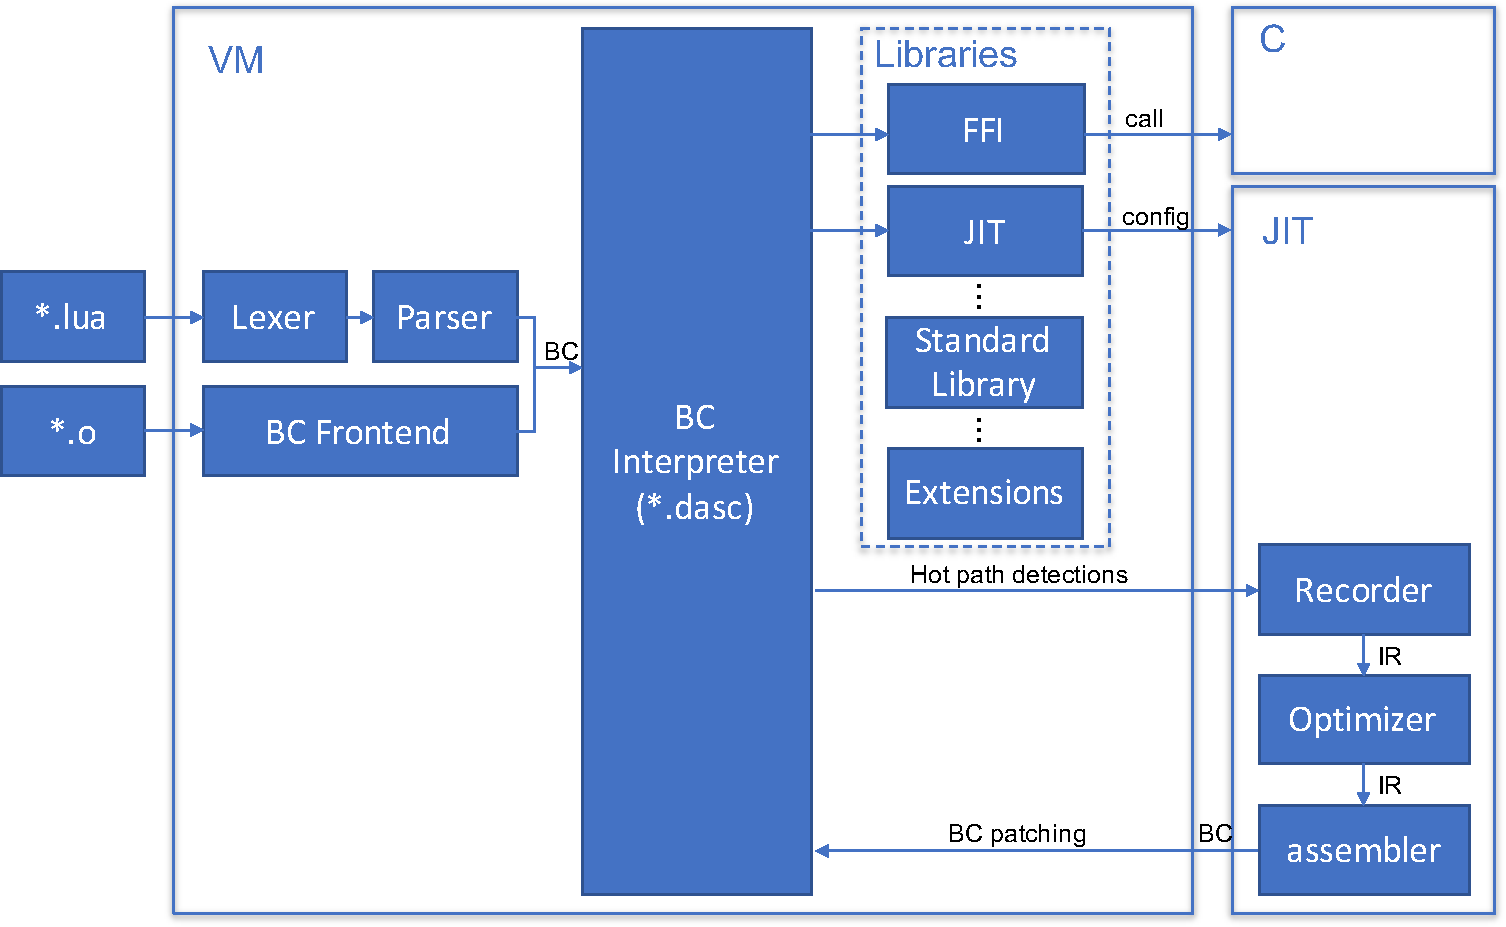
\includegraphics[width=\textwidth]{./Images/LuaJIT.pdf}
    \caption{Schematic view of LuaJIT internals}
    \label{fig:luajit-internal}
\end{figure}{}

First you need to provide luaJIT, files to execute. It accepts two types of input,
text files containing lua code or already converted object files. Lua files are
first read by the \emph{Lexer} \ref{Subsec:Lexer} and \emph{Parser} \ref{Subsec:Parser} and
converted in LuaJIT's bytecode instructions (BC). The other possibility is to provide
object files that contain bytecodes already converted by LuaJIT used for
embedding code in binaries for examples. Those last files are read by the
\emph{bytecode frontend} \ref{Subsec:bc-frontend}.

Once the source code as been converted in bytecode, it is fed to the \emph{bytecode
interpreter} \ref{Sec:BI}. It is the central piece of code written in assembly
that connect every component of luaJIT and is responsible for executing the BC.

There is a certain number of libraries \ref{Sec:Library} packaged will luaJIT, here
to help the BC interpreter to do its work. We will mention a few of them here.
First there is the \emph{FFI} \ref{Sec:FFI} library that allows to directly connect lua
code with c code and c library without lua explicit c interface. The \emph{standard
library} provides a explicit \emph{C} interface to manipulate lua data
(stack, registry, GCObject etc...). Finally, the \emph{JIT} library provides functions
allowing to configure the JIT engine.

The last big part of luaJIT is obviously the \emph{JIT} engine \ref{Chapt:JIT}.
It is actually a tracing JIT that needs to detect \emph{hot path}
\ref{Subsec:hot-path} that would benefit from being compiled. Once such a piece
of bytecode is detected the \emph{recorder} specialize this bytecode with runtime
data and type information and generate an \emph{Intermediate Representation}
equivalent \ref{Subsec:IR}. Then the Optimizer \ref{Sec:TO} modify the IR by
applying a bunch of optimizations on it. Finally, the \emph{assembler} \ref{Sec:TA}
transform the IR into a platform-specific executable binary and the BC that was
detected to be hot is patched to replace his execution to a call to the
corresponding compiled trace.


    \section{Problem description}
    \label{Sec:Problem-description}
    %!TEX root = ../../../FYP_Dissertation.tex

Figure \ref{fig:pb-statement} below shows the time in seconds taken by running 10
times the MAD test suite made of supposedly deterministic code. Surprisingly the
result shows a big variance in performance with the worst case taking more than
12 times the best one. This kind of instability would be unacceptable in the
context of demanding scientific computation here at CERN for the final version
of MAD-NG (currently in early development).

\begin{figure}[H]
    \centering
	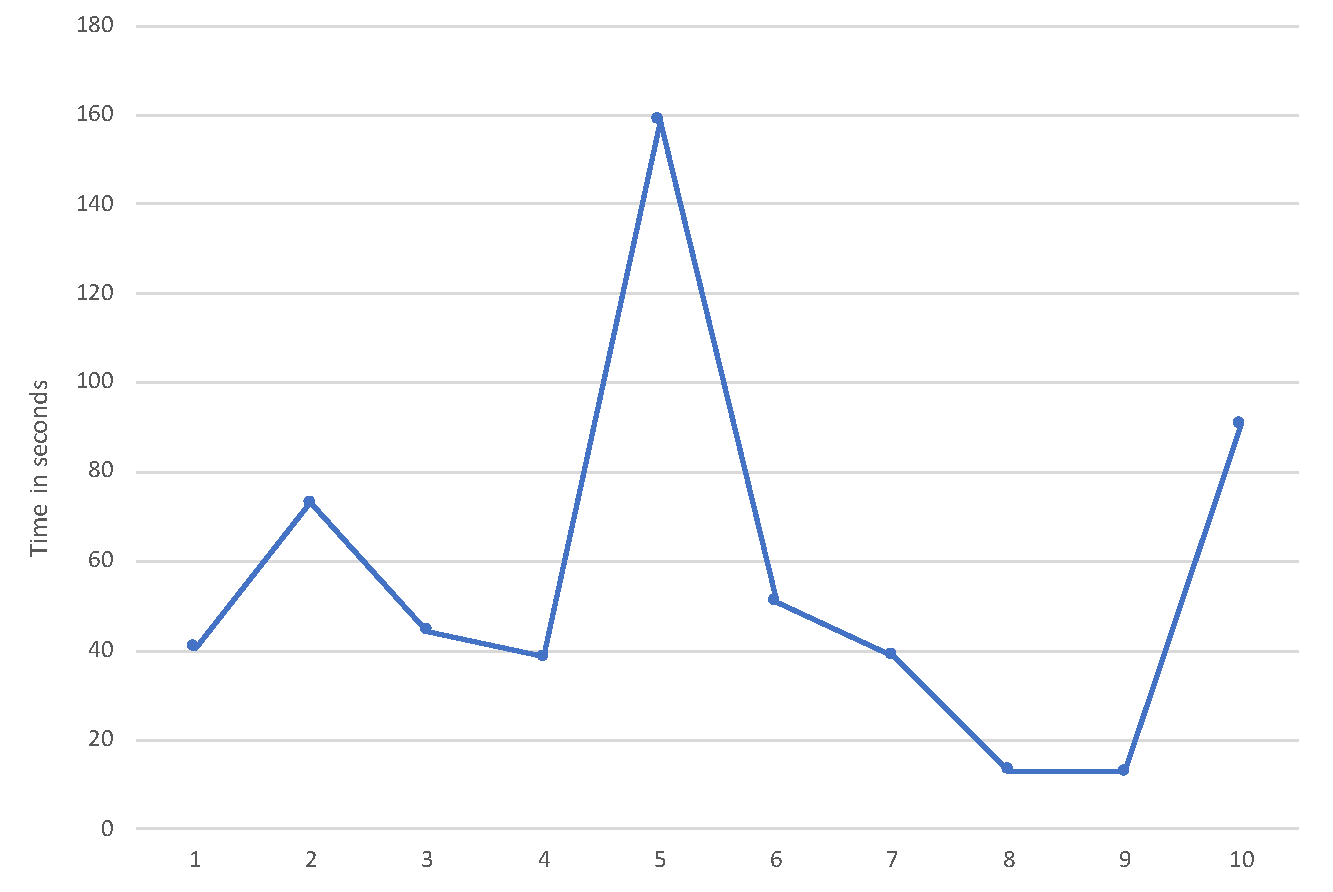
\includegraphics[height=6cm]{./Images/pb-statement-curve.pdf}
	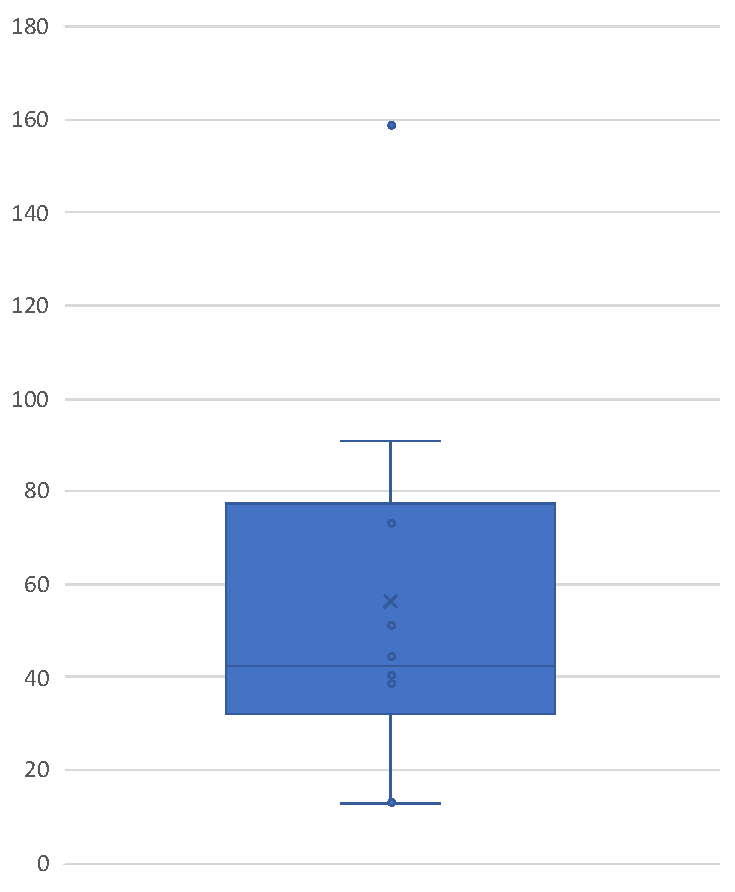
\includegraphics[height=6cm]{./Images/pb-statement-box.pdf}
    \caption{Multiple runs of the same deterministic unit test suite}
    \label{fig:pb-statement}
\end{figure}

The first issue while trying to understand those results is the need of tools
to investigate what is going on under the hood. The second issue is by the
nature of LuaJIT (mostly a one-man job) the documentation is very thin and a bit
scattered all over the place (wiki, website, mailing list, etc.), making life
difficult for newcomers to understand its mechanism.
This is where this project takes place. This part will present analysis of those
instability and provide potential pistes of explanation, while the second part
will present my technical understanding of LuaJIT in a structured way to allow
it to be used as a reference for future newcomers, internally at CERN or for any
interested people.


  \chapter{Model Object}
  \label{Chapt:MO}
  %!TEX root = ../../FYP_Dissertation.tex

When looking at the timing of individual tests of the MAD test suite we can see
that most of the instability comes from the Model Object tests. In Figure
\ref{fig:failed-test}, we can see a screenshot of three failed timing tests that
were calibrated to run in roughly 0.5 seconds and that for this run needed respectively
6, 4 and 68 seconds. We need then to investigate the reason for such results.

\begin{figure}[H]
    \centering
	\includegraphics[width=0.8\textwidth]{./Images/failed-test.png}
    \caption{Timing screenshot}
    \label{fig:failed-test}
\end{figure}

The Lua programming language doesn't actually have an object model but provide
mechanisms that allow anyone to build a custom object model fitting his needs.
Next section will present the one that as been built for MAD.

%===============================================================================
% Model object description
%===============================================================================

\section{Model object description}
\label{Sec:MO-descriptinon}

MAD object module implements the necessary machinery to support prototype-based
programming. When reading an attribute on an object, either the value is present
in the child object and it is returned or the query is passed to the parent
object recursively until the value is found or the original \emph{Object} is
reached. When a value is written the value is simply stored in the current
object (no lookups are performed). To understand how this object model is
implemented, a grasp of how lua handles tables and metatables is required.

To keep it simple here, lua tables are key-value stores that return \emph{nil} by
default if a key is not defined (see Section \ref{Subsec:table} for more).
Users have the possibility to associate a metatable to any tables. A metatable
is actually a standard lua table that contains special metamethods of which
the keys are defined by the lua language. The one that we are interested here is
the \emph{\_\_index} metamethod that defines how a table should react when accessing
an undefined key. If this is a method, the requested key is passed to this method
and it is executed, but if this \emph{\_\_index} contains another table, then this
table is queried instead of the first one. This is this mechanism that has been
used in MAD to implement the model object. Figure \ref{fig:MO-descriptinon} below
shows a schematic of the implementation of MAD object model.

\begin{figure}[H]
    \centering
    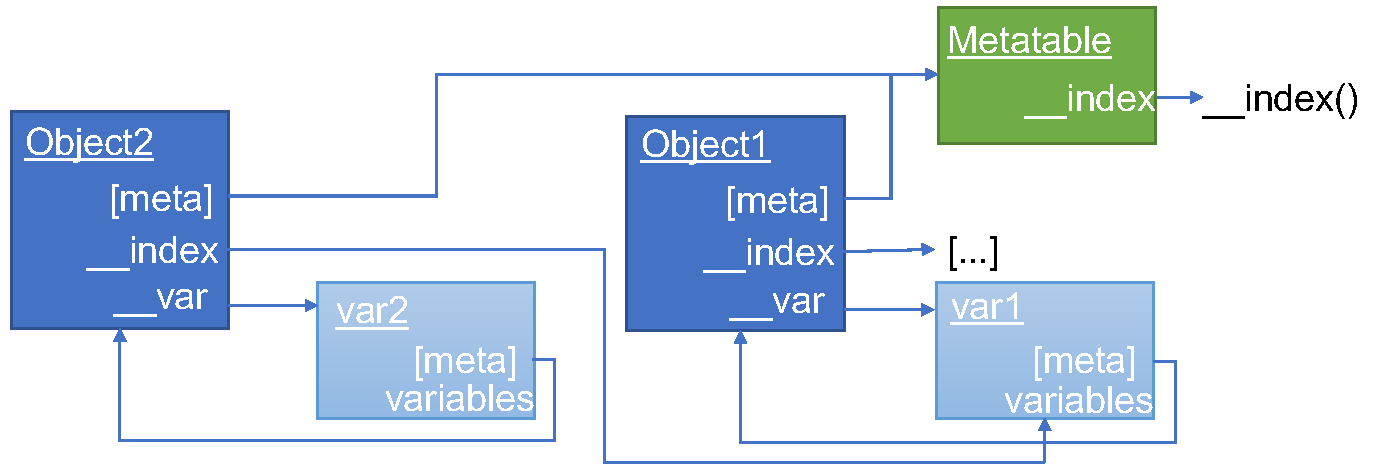
\includegraphics[width=\textwidth]{./Images/MO.pdf}
    \caption{Implementation of MAD object model}
    \label{fig:MO-descriptinon}
\end{figure}

On this figure, \emph{Object2} is the child of \emph{Object1}. To represent an
object, three lua tables are actually needed. The first one (in dark blue) is
the actual object passed around and manipulated by the user. It doesn't actually
contain any user data so when queried, the index function of its metatable (in
green) is executed instead. This metatable is by default the same for all objects
unless it is explicitly modified by the user. This index function gets the
\emph{var} table (in light blue) of the object and try to index it with the
requested key. If the key is defined, the corresponding value is returned,
otherwise the chaining lookup is triggered. Let's look at the example in the
figure when trying to query an undefined key in \emph{Object2}.
First the index function query \emph{var2} that doesn't contain it. Then, since
\emph{Object2} is the metatable of \emph{var2} (see the \emph{[meta]} arrow) and
the \emph{\_\_index} of \emph{Object2} links to \emph{var1}, \emph{var1} is queried.
This chaining is done recursively to the \emph{var} tables of its parents until the
key is found or the hierarchy entirely unrolled.

%===============================================================================
% Performance analysis
%===============================================================================

\section{Performance analysis}
\label{Sec:MO-perf-analys}

First of all, we are going to see how the JIT can make this object model
efficient and hoist away  all those costly lookups. In fact, the object model
described in the previous section might seem very slow as accessing variables
provided by a distant parent necessitates a big chain of lookups. In practice it
is not necessarily the case. Let's look at an example. Figure \ref{fig:MO-ex}
shows a model hierarchy that is transcribed in MAD by the lua code below from
lines 3 to 9. Since LuaJIT mainly compile loops, we are going to look at the IR
code (see Section \ref{Subsec:IR}) generated by LuaJIT for the loop lines 12 to 14
using the dump module (see Section \ref{Sec:Dump-mode}).

\begin{figure}[H]
    \centering
    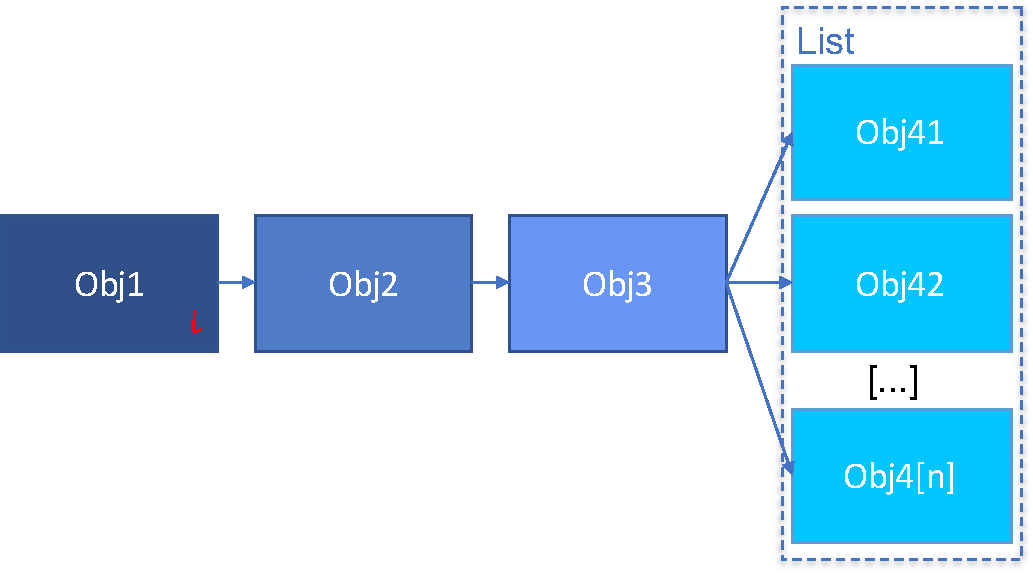
\includegraphics[width=0.8\textwidth]{./Images/MO-ex.pdf}
    \caption{Object inheritance of the example}
    \label{fig:MO-ex}
\end{figure}

\begin{lstlisting}[style=LuaStyle]
local object in MAD

-- object hierarchy
local obj1  = object "obj1"  { l = 42 }
local obj2  = obj1   "obj2"  { }
local obj3  = obj2   "obj3"  { }
local obj41 = obj3   "obj41" { }
local obj42 = obj3   "obj42" { }

-- loop
local sum = 0
for i=1,1e7 do
	sum = sum + obj41.l + obj42.l
end
\end{lstlisting}

\begin{figure}[H]
    \centering
    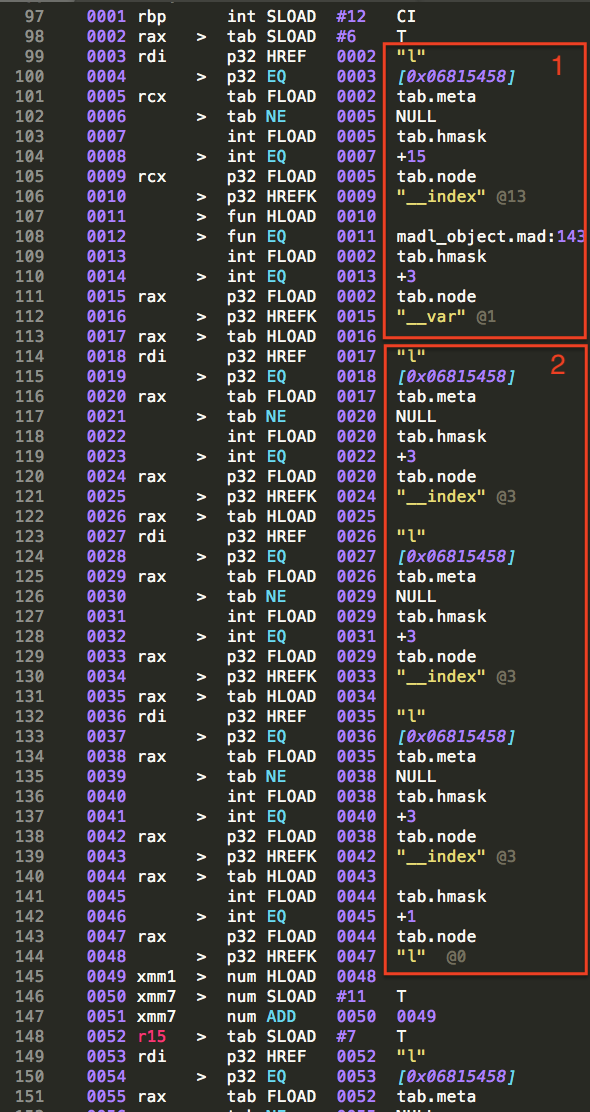
\includegraphics[height=13cm]{./Images/trace-1a}
    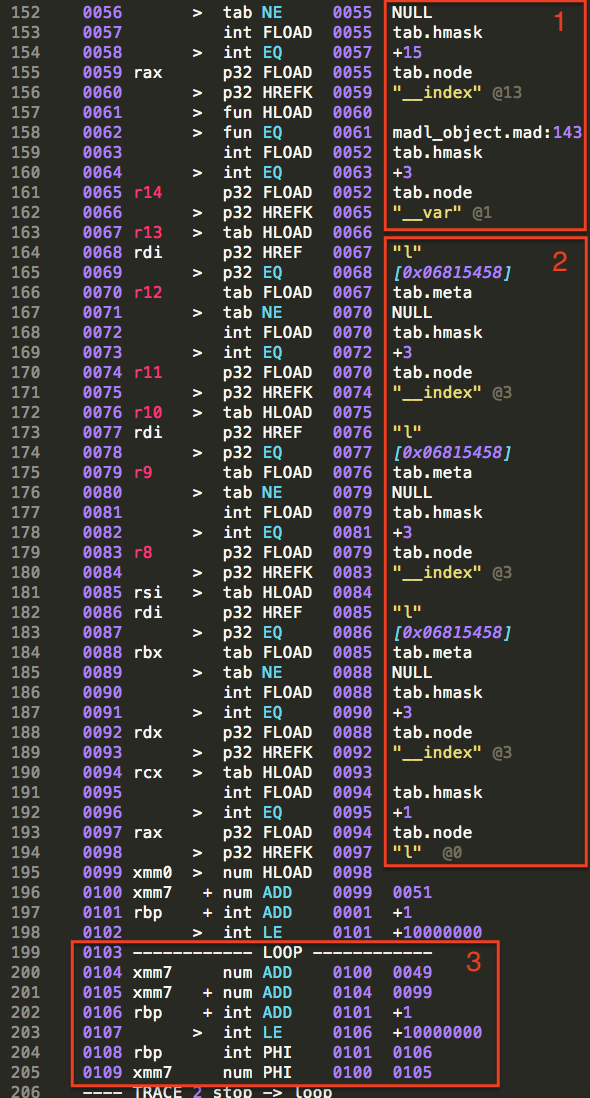
\includegraphics[height=13cm]{./Images/trace-1b}
    \caption{Screenshot of the example's loop trace}
    \label{fig:MO-ex-dump}
\end{figure}

Figure \ref{fig:MO-ex-dump} shows a screenshot of the dump trace. Without looking
at it too much in detail, we can see in the red squares labeled number one, the
access to the \emph{\_\_index} function that access the \emph{\_\_var} table to
query the "l" variable. Since this variable is not present in the first object
the hierarchy is unrolled three time (see the 3 "l" literals and the three
"\emph{\_\_index}" literals) in the red squares labeled with the number 2.
We have twice the same unrolling because the left screenshot shows the
unrolling for the first object (\emph{obj41}) and the right one shows the second
object (\emph{obj42}).

Now let's extract some general understanding from this example. Fist, the actual loop
is only the part in red labeled with the number three. We can see that it only
consists of the loop's counter and the additions. All other operations
from the model object has been successfully moved out of the loop making the loop
itself very small and efficient. This is the power of luaJIT. It can do that
using the loop optimization that consists of unrolling the loop once before the
actual loop itself executing all invariant operation and guards only once
(see \ref{Subsec:opt-loop} on loop optimization). Another thing to note here is
that the hierarchy chaining and the \emph{\_\_index} function is completely
inlined in the trace. This is always the case, there is never any explicit
control-flow possible in a trace with the exception of the actual LOOP currently
recorded, meaning that all functions and control-flow are inlined and specialized
to the runtime values.\\

Now let's look at another example based on the same hierarchy but slightly more
complex. Here the last level objects (\emph{obj4[n]}) are dynamic. Figure
\ref{fig:MO-ex-dump2} shows a screenshot of the dump trace for the second
example and we can clearly see that the hierarchy chaining is present both before
the loop (on the left) and inside the loop (on the right). This means that the
compiler hasn't been able to detect the invariance and produce a code similar to
the previous example, but it still manages to produce a single trace handling the
entire loop making it still performing better than with the VM interpreter.

\begin{lstlisting}[style=LuaStyle]
local object in MAD

-- object hierarchy
local obj1 = object "obj1" { l = 42 }
local obj2 = obj1   "obj2" { }
local obj3 = obj2   "obj3" { }

-- list of obj4[n]
local list = table.new(1e7, 0)
for i=1,1e7 do
	lists[i] = obj3 "obj4" {}
end

-- loop
local sum = 0
for i=1,1e7 do
	sum = sum + lists[i].l
end
\end{lstlisting}

\begin{figure}[H]
    \centering
    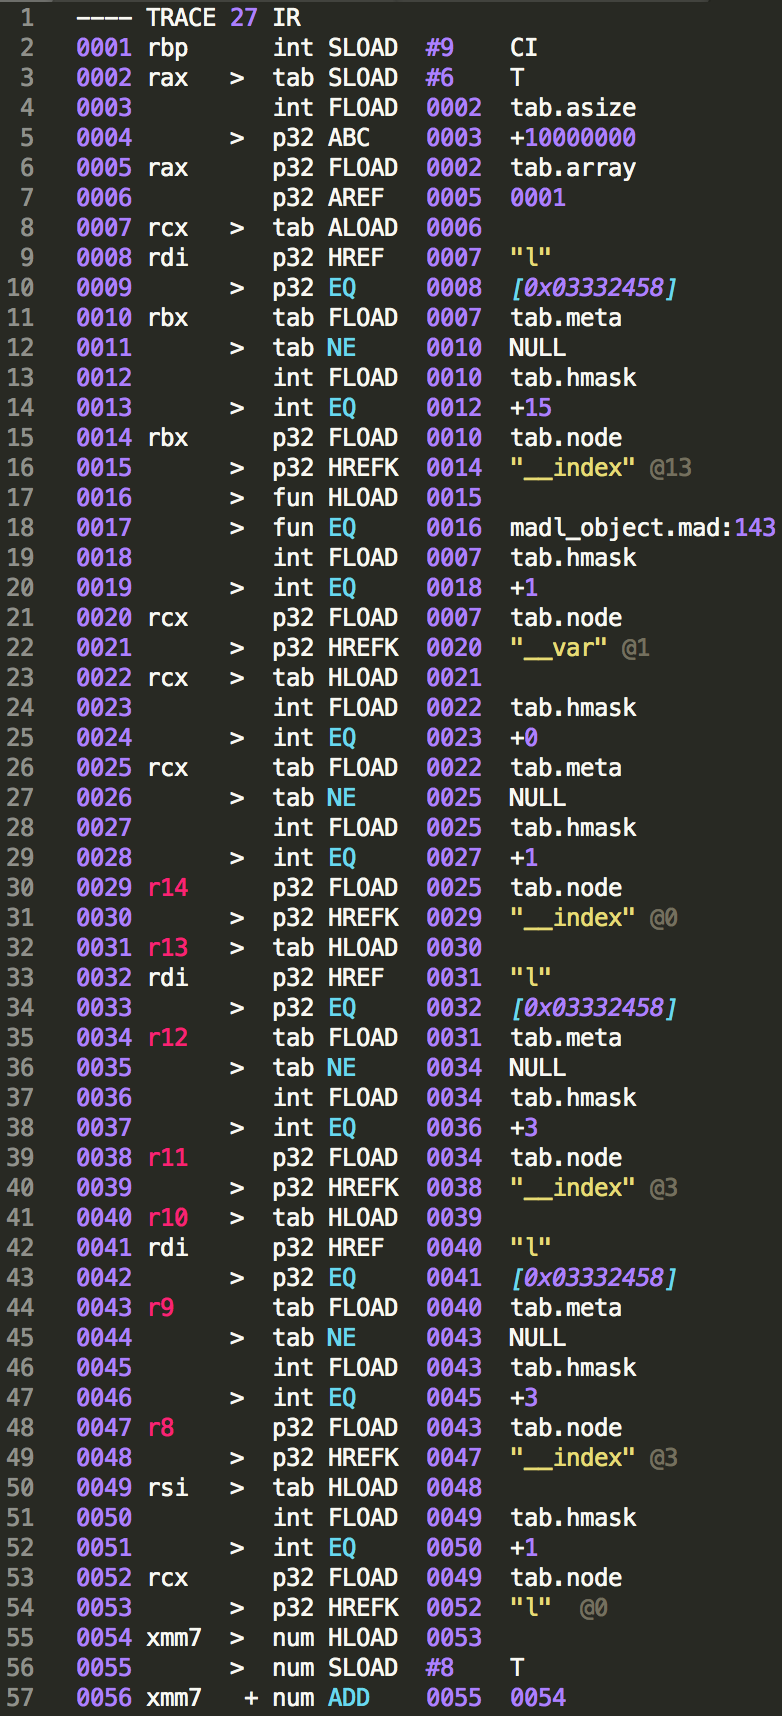
\includegraphics[height=13cm]{./Images/trace-2a}
    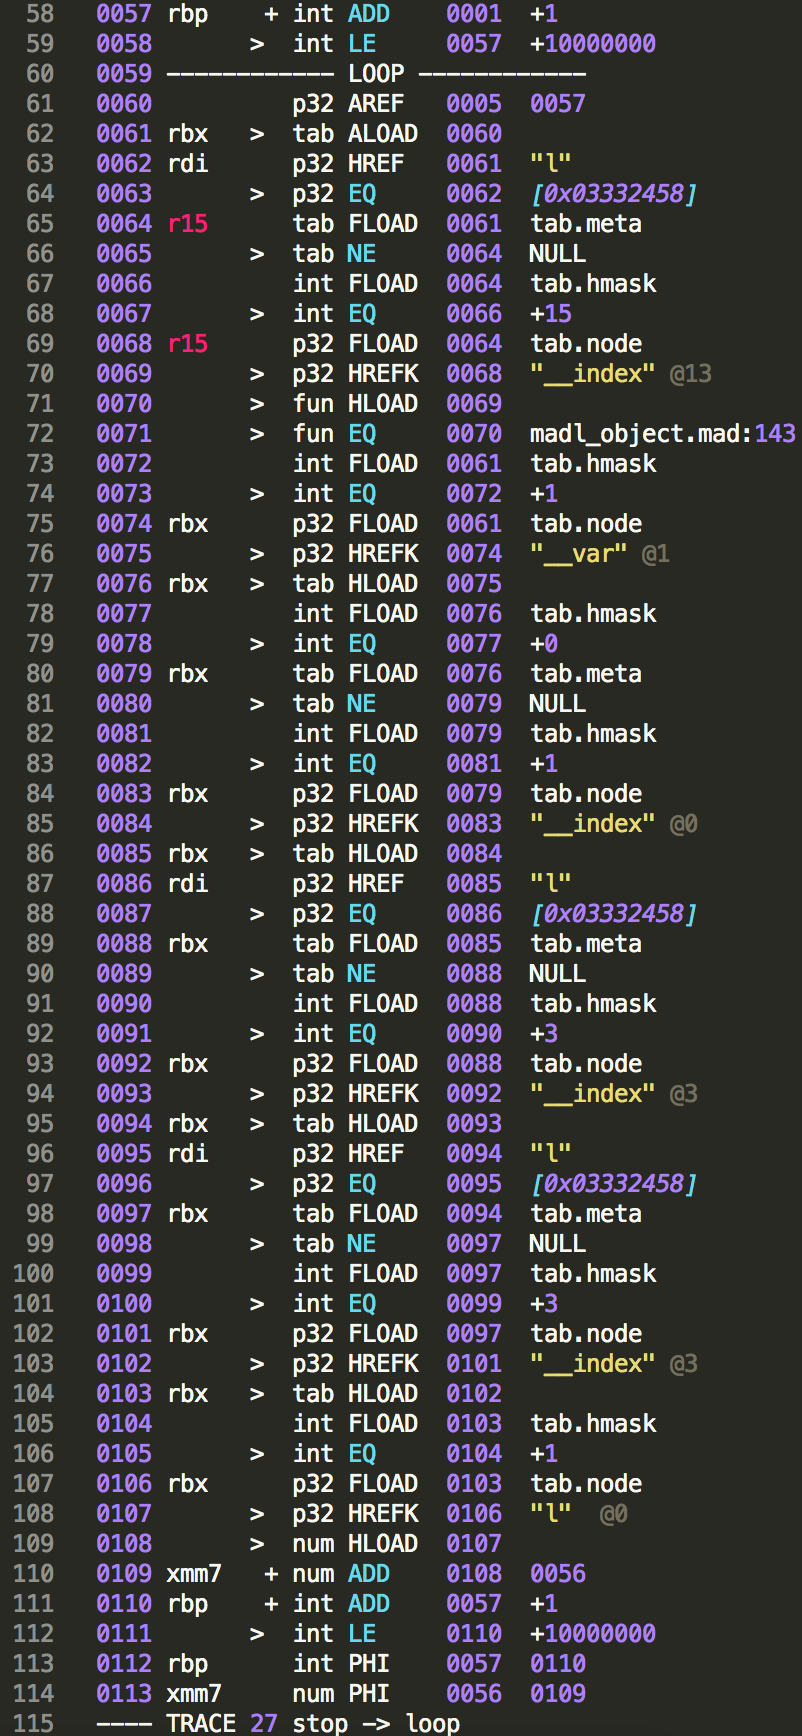
\includegraphics[height=13cm]{./Images/trace-2b}
    \caption{Screenshot of the second example's loop trace}
    \label{fig:MO-ex-dump2}
\end{figure}

%===============================================================================
% Instability possible explanation
%===============================================================================

\section{Possible explanations for performance hit}
\label{Sec:MO-insta}

The first thing interesting to note is that we can deactivate the JIT engine using
the \emph{-joff} command-line argument of LuaJIT and we can see that the VM is
slightly faster than the worst case scenario with the JIT activated. This can
be explained by the fact that in those cases the actual code is entirely run by
the VM, plus the compiler spent some time trying to record and generate traces
that end-up being aborted. Those claim can be verified by using the \emph{v}
option of the profiler (see Section \ref{Sec:Profiler}). The question now is :
why is it, that so much time is spent in the VM and why all those trace gets
aborted. This is where things gets complicated. When run stand-alone the
performance test mentioned earlier are always perfectly fine. It is depending of
the context, meaning the code that has been run before, that sometime makes those
test take a incredible amount of time. In addition of that the dump module of
LuaJIT is very useful when we want to study isolated problems but in this case
where the amount of code run influence the result, this tool generate to much
informations without much help to manipulate them, making it a needle in a
haystack kind of problem.\\

We will still present here some insight on this issue with some unsuccessful
tentative of solutions.

The first thing is that in some run the \emph{\_\_index}
function of the model object (presented in previous sections) gets blacklisted
(see Section \ref{Subsec:abort}). After that no hierarchy chaining can be
successfully recorded inside another trace making all of them running
exclusively in the VM. This is due to a mechanism of LuaJIT that we can call
\emph{cascading blacklisting} that consist of blacklisting bytecode that tries to
record a trace that hit another blacklisted bytecode. This is very inconvenient
because it means that a piece of code that can't be properly compiled for
whatever the reason can make the model object very slow for the rest of the run.
This is even more problematic knowing that blacklisting is permanent for the
lifetime of a particular bytecode, making it in this case for an entire run of
LuaJIT.

A second interesting fact to try to explain the instability part of the problem
is the fact that the hot path detection is very lazy and use the hashed program
counter (see Section \ref{Subsec:hot-path}) making false positive very easy to
occur. So any change to the code can change the bytecode alignment and the
potential false positive, changing in its turn the entire profile of the code
generated. This explanation is an educated guess and couldn't be formally proven
to be explaining in its own the change of behavior seen when slightly modifying
codes.

Another thing to consider is that in LuaJIT strings are internalized (see
Section \ref{Subsec:string-inter}) and that the memory address where they are
stored is used has "identifier" for string comparisons or hash-table placements.
Due to the ASLR (Address Space Layout Randomization) of many operating systems,
two consecutive runs of the exact same code will generate different address for
internalized string and possibly different placement inside hash-tables. In Lua
iterating over a hash-table can be done through the \emph{pairs} iterator that
doesn't enforce any special order (it just iterate sequentially over the internal
table structure), thus two runs can result in keys not being read in the same order,
making the JIT "see" the codes in a different order possibly changing false positive
and other behavior of the JIT.\\

Now let's have a look at a few modifications of LuaJIT that has been done to try
to circumvent the blacklisting problem. The first idea was that blacklisting
should be context specific, so any compiler wide trace flush (that we can
internally detect) should walk through the bytecode resetting the flag to any
blacklisted function or loop-like bytecode. The second idea was two slightly
change the behavior of this \emph{cascading blacklisting} feature by letting
traces record over blacklisted bytecode instead of aborting immediately.
Unfortunately those two tried modifications didn't bring any substantial
improvement over stability or performance. They can still be a nice idea to keep
in mind and might be reintroduced letters.

%===============================================================================
% Performance of Sequence iterator
%===============================================================================

\section{Performance of \emph{Sequence} iterator}
\label{Sec:MO-perf-iter}

% forward vs backward iterator
% difference in performance
% comming from the nedd of the l
	% different depth to get l
	% show a visual dump
% new object model ?
% loop optimization is a problem here when the list is heterogenous in numbers of stages
%  permanant blacklisting

%===============================================================================
% Model object alternative design
%===============================================================================

\section{Alternative design of the model object}
\label{Sec:MO-alt-design}

% exploration of other type of object model
%  performance compareson / explanation
% didn't help on average


  % \chapter{Sequence}
  % \label{Chapt:seq}

  % \chapter{Mtable}
  % \label{Chapt:mtable}

\part{LuaJIT implementation study}
\label{Part:luajit-doc}

  \chapter{Virtual Machine}
  \label{Chapt:VM}

    \section{Frontend}
    \label{Sec:frontend}
    \lhead{Chapter \thechapter. \emph{Frontend}}
    %!TEX root = ../FYP_Dissertation.tex

%===============================================================================
% Lexer
%===============================================================================

\subsection{Lexer}
\label{Subsec:Lexer}

The lexer is implemented in the \emph{lj\_lex.c} and \emph{lj\_lex.h} files.
It use \emph{LexState} as a principal data structure. The user-provided
\emph{rfunc} function is used to read a chunk of data to process. It is accessed
through the \emph{p} and \emph{pe} pointers. The main function is
\emph{lex\_scan} that dispatches the work to other functions depending of the
type of data to be processed (comment, string literal, long string, numbers
etc...). TValues (\emph{tokval}, \emph{lookaheadval}) are used to store the
token values were \emph{LexToken} (\emph{tok}, \emph{lookahead}) determine the
type. The string buffer (\emph{sb}) is used to accumulate characters of a future
string before internalizing it. All lua keyword are internalized as a string at
the very beginning, GCstr has the field \emph{reserved} for marking them.

\begin{lstlisting}[style=CStyle]
typedef struct LexState {
  struct FuncState *fs; /* Current FuncState. Defined in lj_parse.c. */
  struct lua_State *L;  /* Lua state. */
  TValue tokval;        /* Current token value. */
  TValue lookaheadval;  /* Lookahead token value. */
  const char *p;        /* Current position in input buffer. */
  const char *pe;       /* End of input buffer. */
  LexChar c;            /* Current character. */
  LexToken tok;         /* Current token. */
  LexToken lookahead;   /* Lookahead token. */
  SBuf sb;              /* String buffer for tokens. */
  lua_Reader rfunc;     /* Reader callback. */
  void *rdata;          /* Reader callback data. */
  BCLine linenumber;    /* Input line counter. */
  BCLine lastline;      /* Line of last token. */
  GCstr *chunkname;     /* Current chunk name (interned string). */
  const char *chunkarg; /* Chunk name argument. */
  const char *mode;     /* Allow loading bytecode (b) and/or source text (t). */
  VarInfo *vstack;      /* Stack for names and extents of local variables. */
  MSize sizevstack;     /* Size of variable stack. */
  MSize vtop;           /* Top of variable stack. */
  BCInsLine *bcstack;   /* Stack for bytecode instructions/line numbers. */
  MSize sizebcstack;    /* Size of bytecode stack. */
  uint32_t level;       /* Syntactical nesting level. */
} LexState;
\end{lstlisting}

%===============================================================================
% Parser
%===============================================================================

\subsection{Parser}
\label{Subsec:Parser}

The parser of luaJIT is implemented in \emph{lj\_parse.c} and \emph{lj\_parse.h}
files. it also use \emph{LexState} as the principal data-structure. it is the on
responsible for calling the lexer to get tokens. LuaJIT doesn't really have an
abstract syntax tree representation of the parsed code. Instead it directly
generates the bytecode on the fly using helpers from \emph{lj\_bc.h}.
The \emph{lj\_parse} function is the entry point and parse the main chunck as a
vararg function. The unit of emission is the function (\emph{GCproto}) and the structure used for the construction is \emph{FuncState}. Parsing is a succession
of chuncks (\emph{parse\_chunk}) were \emph{parse\_stmt} is the principal
function called for each line, dispatching the work depending of the current
token type. \emph{FuncScope} is a linked-list of structure used for scope
management.

\begin{lstlisting}[style=CStyle]
typedef struct FuncState {
  GCtab *kt;              /* Hash table for constants. */
  LexState *ls;           /* Lexer state. */
  lua_State *L;           /* Lua state. */
  FuncScope *bl;          /* Current scope. */
  struct FuncState *prev; /* Enclosing function. */
  BCPos pc;               /* Next bytecode position. */
  BCPos lasttarget;       /* Bytecode position of last jump target. */
  BCPos jpc;              /* Pending jump list to next bytecode. */
  BCReg freereg;          /* First free register. */
  BCReg nactvar;          /* Number of active local variables. */
  BCReg nkn, nkgc;        /* Number of lua_Number/GCobj constants */
  BCLine linedefined;     /* First line of the function definition. */
  BCInsLine *bcbase;      /* Base of bytecode stack. */
  BCPos bclim;            /* Limit of bytecode stack. */
  MSize vbase;            /* Base of variable stack for this function. */
  uint8_t flags;          /* Prototype flags. */
  uint8_t numparams;      /* Number of parameters. */
  uint8_t framesize;      /* Fixed frame size. */
  uint8_t nuv;            /* Number of upvalues */
  VarIndex varmap[...];   /* Map from register to variable idx. */
  VarIndex uvmap[...];    /* Map from upvalue to variable idx. */
  VarIndex uvtmp[...];    /* Temporary upvalue map. */
} FuncState;
\end{lstlisting}

%===============================================================================
% Bytecode frontend
%===============================================================================

\subsection{Bytecode frontend}
\label{Subsec:bc-frontend}

Another frontend feature provided by luaJIT is the possibility to save and load
bytecode directly, allowing to skip the lexer and parser phase.

The writing part is handled by the module \emph{bcsave.lua} that use the
\emph{lj\_bcwrite} function from \emph{lj\_bcwrite.c} to generate the data to be written.

The reading part is done by the code in \emph{lj\_bcread.c} file. When it is
detected that the input file is a bc dump instead of a plain lua code,
\emph{cpparser} from \emph{lj\_load.c} calls \emph{lj\_bcread} instead of
\emph{lj\_parse} normally. This reader also use \emph{LexState} as the principal
data-structure.



    \section{Internals}
    \label{Sec:Internals}
    \lhead{Chapter \thechapter. \emph{Internals}}
    %!TEX root = ../FYP_Dissertation.tex

%===============================================================================
% Tagged value
%===============================================================================

\subsection{Tagged value}
\label{Subsec:tagged-value}

LuaJIT represent all internal element as 64-bits \emph{TValue} (tagged value).
It use the nan-tagging technique to differentiate between numbers and other
types of element. In fact, \emph{lua\_number} are 64-bits floating-points numbers
following the \emph{ieee} standard. Doing so, numeric nan are canonized by the
cpu FPU (0xfff8 in msb and zero otherwise), letting the possibility to use the
lower bits to represent arbitrary data. Internally, LuaJIT has two different
representations, one for x86 and another for x64 bit (\emph{LJ\_GC64}) mode
(see Table \ref{tab:tagged-gc32} and \ref{tab:tagged-gc64}). In those table,
\emph{itypes} are numbers identifying the type of the object.
GC object (Garbage Collectible Object) represent all allocated object
that are managed by the garbage collector. \emph{GCRef} are references to such
object.

\begin{table}[H]
\centering
\caption{Internal object tagging for 32-bits mode}
\label{tab:tagged-gc32}
\begin{tabular}{l|c|c|c|}
\cline{2-4}
                                              & \multicolumn{2}{c|}{MSW}         & LSW         \\ \hline
\multicolumn{1}{|l|}{size}                    & \multicolumn{2}{c|}{32-bits}     & 32-bits     \\ \hline
\multicolumn{1}{|l|}{primitive types}         & \multicolumn{2}{c|}{itypes}      &             \\
\multicolumn{1}{|l|}{lightuserdata (32-bits)} & \multicolumn{2}{c|}{itypes}      & void *      \\
\multicolumn{1}{|l|}{lightuserdata (64-bits)} & 0xffff           & \multicolumn{2}{c|}{void *} \\
\multicolumn{1}{|l|}{GC objects}              & \multicolumn{2}{c|}{itypes}      & GCRef       \\
\multicolumn{1}{|l|}{int}                     & \multicolumn{2}{c|}{itypes}      & int         \\
\multicolumn{1}{|l|}{number}                  & \multicolumn{3}{c|}{double}                    \\ \hline
\end{tabular}
\end{table}

\begin{table}[H]
\centering
\caption{Internal object tagging for 64-bits mode}
\label{tab:tagged-gc64}
\begin{tabular}{l|c|c|c|c|}
\cline{2-5}
                                      & \multicolumn{3}{c|}{MSW}         & LSW         \\ \hline
\multicolumn{1}{|l|}{size}            & 13-bits & 4-bits & 15-bits       & 32-bits     \\ \hline
\multicolumn{1}{|l|}{primitive types} & 1...1   & itype  & \multicolumn{2}{c|}{1...1}  \\
\multicolumn{1}{|l|}{lightuserdata}   & 1...1   & itype  & \multicolumn{2}{c|}{void *} \\
\multicolumn{1}{|l|}{GC objects}      & 1...1   & itype  & \multicolumn{2}{c|}{GCRef}  \\
\multicolumn{1}{|l|}{int}             & 1...1   & itype  & 0...0         & int         \\
\multicolumn{1}{|l|}{number}          & \multicolumn{4}{c|}{double}                    \\ \hline
\end{tabular}
\end{table}

%===============================================================================
% String Internalization
%===============================================================================

\subsection{String Internalization}
\label{Subsec:string-inter}

All strings that are manipulated by LuaJIT are internalized. This includes, all
the strings literals of the user lua code, all identifier and tokens of the lua
code itself and also all the strings used internally by LuaJIT. Internalization
mechanism does that, only one copy of a specific strings is kept in memory. If
multiple copy of a same string are requested, a pointer to the internalized
version of the string is returned, instead of doing a new string allocation.
Strings need to be immutable and are zero-terminated. Strings function are
implemented in the \emph{lj\_str.c} file and internalization is done by the
\emph{lj\_str\_new} function.

For that, it implements a hash table and use a very sparse but fast hash
function. Collisions are handled by the use of singly-chained linked list.
The table is resized and all string rehashed when a 100\% load is reached.
The necessary states are saved in the \emph{global\_State} structure in the
\emph{lj\_obj.h} file.

\begin{lstlisting}[style=CStyle]
typedef struct global_State {
  GCRef *strhash; /* String hash table (hash chain anchors). */
  MSize strmask;  /* String hash mask (size of hash table - 1). */
  MSize strnum;   /* Number of strings in hash table. */
  [...]
}
\end{lstlisting}

%===============================================================================
% Lua table
%===============================================================================

\subsection{Lua table}
\label{Subsec:table}

Tables are garbage collectible objects represented by the structure bellow
(\emph{GCtab} in \emph{lj\_obj.h}). Functions to manipulate them are in
\emph{lj\_tab.c} and \emph{lj\_tab.h} files. It is composed of an array part and
a hash part. If the array part is small, it is allocated directly after the
structure in memory (collocation functionality), otherwise it is separated. The
hash part is a hash table used to store all non-integer key (or integer too big
to fit in the array part). It is implemented has an array using singly-linked
list for collision, where nodes of the linked list are within the array (not
allocated) and a variation of \emph{Brent's hashing methods} is used.
New integer key that are bigger than the array part are always inserted
in the hash part until this one is full. It then trigger the resizing of the
table. The new \emph{asize} and \emph{hmask} are both power of 2. The
new \emph{asize} value correspond to the biggest power of 2 such that at least
50 percent of the integers bellow it are used as key. The new \emph{hmask} is
picket such that all non-integer keys plus the integer keys that are bigger than
the new \emph{asize} fit in it. When a resizing occur the hash values are
re-hashed and integer key that does fit now in the array part are reintroduce
there.

The \emph{nomm} field of GCtab is a
negative cache for fast metamethods checks. It is a bitmap marking absent fields
of the metatable.

\begin{lstlisting}[style=CStyle]
typedef struct GCtab {
  GCHeader;
  uint8_t nomm;    /* Negative cache for fast metamethods. */
  int8_t colo;     /* Array colocation
  (number of slot directly following in memory).*/
  MRef array;      /* Array part. */
  GCRef gclist;
  GCRef metatable; /* Must be at same offset in GCudata. */
  MRef node;       /* Hash part. */
  uint32_t asize;  /* Size of array part (keys [0, asize-1]). */
  uint32_t hmask;  /* Hash part mask (size of hash part - 1). */
#if LJ_GC64
  MRef freetop;    /* Top of free elements. */
#endif
} GCtab;
\end{lstlisting}

%===============================================================================
% Garbage collector
%===============================================================================

\subsection{Garbage collector}
\label{Subsec:gc}

LuaJIT garbage collector has currently a tri-color, incremental mark and sweep
types implementation. You can find a presentation of it on the wiki
\cite{luajit-gc} in the tri-color section. Its source code can be found in the
\emph{lj\_gc.h} and \emph{lj\_gc.c} files. It uses the GCState structure has a
principal structure. The \emph{gc\_onestep} function is the principal one as it
implement the stat machine of the gc. Principal state with their meaning can be
found in the enum bellow.

\begin{lstlisting}[style=CStyle]
enum {
  GCSpause,
  GCSpropagate,   /* One gray object is processed. */
  GCSatomic,      /* Atomic transition from mark to sweep phase. */
  GCSsweepstring, /* Sweep one chain of strings from the table. */
  GCSsweep,       /* Sweep a few object from root. */
  GCSfinalize     /* Finalize one userdata or cdata object. */
};
\end{lstlisting}

\begin{lstlisting}[style=CStyle]
typedef struct GCState {
  GCSize total;         /* Memory currently allocated. */
  GCSize threshold;     /* Memory threshold. */
  uint8_t currentwhite; /* Current white color. */
  uint8_t state;        /* GC state. */
  uint8_t nocdatafin;   /* No cdata finalizer called. */
  uint8_t unused2;
  MSize sweepstr;       /* Sweep position in string table. */
  GCRef root;           /* List of all collectable objects. */
  MRef sweep;           /* Sweep position in root list. */
  GCRef gray;           /* List of gray objects. */
  GCRef grayagain;      /* List of objects for atomic traversal. */
  GCRef weak;           /* List of weak tables (to be cleared). */
  GCRef mmudata;        /* List of userdata (to be finalized). */
  GCSize debt;          /* Debt (how much GC is behind schedule). */
  GCSize estimate;      /* Estimate of memory actually in use. */
  MSize stepmul;        /* Incremental GC step granularity. */
  MSize pause;          /* Pause between successive GC cycles. */
} GCState;
\end{lstlisting}

%===============================================================================
% Allocator
%===============================================================================

\subsection{Allocator}
\label{Subsec:alloc}

LuaJIT has its own embedded allocator that is a customized version of \emph{dlmalloc}
(Doug Lea's Malloc). Information on the original implementation can be found on
the web article \cite{dlmalloc-art} or in the comment of the code
\cite{dlmalloc-impl}. The allocator is implemented in the \emph{lj\_alloc.c}
file. It's main structure \emph{malloc\_state} is shown bellow. Memory on the
heap are allocated in chunk. Free chunk are managed as double linked-list with
the size of the chunk at the beginning and end of it. Unallocated memory are
grouped in bins of corresponding size. There is two types of bins. The
smaller one contains chunck of same size and the top are anchored in
\emph{smallbins}. The bigger one are stored as bitwise digital tree (aka tries)
keyed by size were the top of a tree is anchored in \emph{treebins}. The
allocator differentiates with two types of memory allocation, if it is higher than
128KB then it ask the operating system for a new memory segment using mmap, if
it is lower than that it use chunks from the current segment. All allocated
segments are kept in a linked list anchored in \emph{seg}. For such smaller
allocation the allocator first try to find an exact fit from the available
chunks to optimize for internal fragmentation. If it cannot find one and that
the requested size is smaller than \emph{dvsize} then it use the \emph{dv}
chunk (designated victim) which is the last chunk that has been split. It does
so to optimize for locality. Otherwise it goes for a best-fit match. If no chunk
big enough is available it ask the system to extend the segment and use the
boundary chunk \emph{top} (kept always free). When memory is freed it does chunk
coalescing to avoid memory fragmentation. If \emph{topsize} is bigger than
\emph{trim\_check}, then the current segment is shrinked and the memory is given
back to the os. \emph{release\_checks} is a decreasing counter that when it
riches zero triggers a check of all segments to release empty ones back to the os.

\begin{lstlisting}[style=CStyle]
struct malloc_state {
  binmap_t  smallmap;       /* marking non-empty smallbins */
  binmap_t  treemap;        /* marking non-empty treebins  */
  size_t    dvsize;         /* designated victim size      */
  size_t    topsize;        /* boundary chunk size         */
  mchunkptr dv;             /* designated victim           */
  mchunkptr top;            /* boundary chunk              */
  size_t    trim_check;     /* threshold size to release   */
  size_t    release_checks; /* counter for mmap release    */
  mchunkptr smallbins[...]; /* anchor for top small bins   */
  tbinptr   treebins[...];  /* anchor for top tree bins    */
  msegment  seg;            /* anchor for chained segments */
};
\end{lstlisting}

%===============================================================================
% Function
%===============================================================================

\subsection{Function}
\label{Subsec:func}

There are two distinct representation for function, the function's prototype,
and the function's closure. the Lua functions' prototypes are represented by \emph{GCproto} (\emph{lj\_obj.h}), and are followed by the functions' bytecodes in memory.
The closures are represented by the GCfuncL for lua function and GCfuncC for
c function (using lua's api). They contains the necessary information for
upvalues. Upvalues are represented by the \emph{GCupval} that if close, contains
the corresponding value or a reference to the stack slot containing the
appropriate value otherwise. Closure can be manage by the functions present in
\emph{lj\_func.c} allowing to create them, destroy them and closing their
upvalues.

\begin{lstlisting}[style=CStyle]
typedef struct GCproto {
  GCHeader;
  uint8_t numparams; /* Number of parameters. */
  uint8_t framesize; /* Fixed frame size. */
  MSize sizebc;      /* Number of bytecode instructions. */
  [...]
  GCRef gclist;
  MRef k;            /* Split constant array (ptr to the middle).*/
  MRef uv;           /* Upvalue list. local slot or parent uv idx. */
  MSize sizekgc;     /* Number of collectable constants. */
  MSize sizekn;      /* Number of lua_Number constants. */
  MSize sizept;      /* Total size including colocated arrays. */
  uint8_t sizeuv;    /* Number of upvalues. */
  uint8_t flags;     /* Miscellaneous flags. */
  uint16_t trace;    /* Anchor for chain of root traces. */
  [...]
} GCproto;
\end{lstlisting}

%===============================================================================
% Fast Function
%===============================================================================

\subsection{Fast Function}
\label{Subsec:ffunc}

Fast functions are specially optimize standard library function. There is two
part for each function, the implementation part and the fallback handler.
The implementation part is done in assembly in the \emph{vm\_*.dasc} files and
handle the general case, called the fast pass. If the fast pass fail, the vm
call the corresponding fallback handler (all \emph{LJLIB\_ASM} marked functions)
that will tries to recover from the failure if possible. Example of recoverable
cases might be : a wrong argument type if coercion succeeds or a stack overflow
if stack reallocation succeeds (see comment in lj\_lib.h).


    \section{Bytecode interpreter}
    \label{Sec:BI}
    \lhead{Chapter \thechapter. \emph{Bytecode interpreter}}
    %!TEX root = ../FYP_Dissertation.tex
Most a the VM mechanism is written using the DynASM syntax. To get a better
understanding of the underlining technology see Appendix \ref{Apendix:DynASM}.

The low-level VM code written for each architecture using this assembler can be
found in \emph{vm\_(target).dasc} files. It is mainly composed of the switch
case that generate the assembly code for each byte code, but it also contains
code for other part that requires low level implementation such as the
stack unwinding or the implementation of the fast path of asm fast library functions
(see section \ref{Subsec:ffunc} for more).

    \section{Library}
    \label{Sec:Library}
    \lhead{Chapter \thechapter. \emph{Library}}
    %!TEX root = ../FYP_Dissertation.tex

%===============================================================================
% Standard library
%===============================================================================

\subsection{Standard library}
\label{Subsec:std-lib}

LuaJIT is providing a full compatibility with Lua 5.1 and to do so, it
implements the standard library. The code is copied and adapted from the
\emph{PUC-RIO} Lua interpreter. A list of the corresponding files and the
descriptions of what they are doing can be found in table
\ref{tab:library-std-files}.

\begin{table}[H]
\centering
\caption{Implementation's files of the Lua standard library}
\label{tab:library-std-files}
\begin{tabular}{|l|l|}
\hline
\multicolumn{1}{|c|}{File name} & \multicolumn{1}{c|}{Description}                     \\ \hline
lib\_base.c                     & Base and coroutine library.                          \\
lib\_debug.c                    & Debug library.                                       \\
lib\_init.c                     & Load and initialize standard libraries.              \\
lib\_io.c                       & Files and I/O library.                               \\
lib\_math.c                     & Math library (abs, sqrt, log, random, etc...).       \\
lib\_os.c                       & OS library (date, time, execute, remove, etc...).    \\
lib\_package.c                  & Package library (load, require, etc...).             \\
lib\_string.c                   & String library (gsub, match, etc...).                \\
lib\_table.c                    & Table library (new, clear, insert, foreach, etc...). \\ \hline
\end{tabular}
\end{table}

%===============================================================================
% LuaJIT extensions
%===============================================================================

\subsection{LuaJIT extensions}
\label{Subsec:lj-extensions}

In addition of the standard library, luaJIT comes equipped with some library
extensions \cite{extensions}. In addition of a few improvements of existing
modules it provides three new extension modules, namely, \emph{bit} in
\emph{lib\_bit.c} that provides with bitwise operations \cite{bitOp}, \emph{ffi}
in \emph{lib\_ffi.c} that provide functions to interact with the FFI library
(see FFI Chapter \ref{Sec:FFI} for more) and \emph{jit} in \emph{lib\_jit.c}
that provide functions allowing to control the behavior of the JIT compiler
engine (see JIT Part \ref{Chapt:JIT}).

%===============================================================================
% The C API
%===============================================================================

\subsection{The C API}
\label{Subsec:c-api}

All those libraries are implemented using the Lua C API that allows to create
and manipulate lua data, manage de lua stack etc... The implementation for those
functions can be found in \emph{lj\_api.c}, \emph{lj\_lib.c} and \emph{lib\_aux.c}.

%===============================================================================
% Build Library
%===============================================================================

\subsection{Build Library}
\label{Subsec:build-lib}

LuaJIT use multiple tricks to generate files automatically that are included
during compilation to help with the building and loading of the standard library
without the need for manual maintenance. We will describe here the different
steps and what they are useful for.

First of all if no lua interpreter
(either PUC-Lua or LuaJIT) is available on the machine a simplified and
minimized one is build from the \emph{minilua.c} file. Then the interpreter is
used to run \emph{genlibbc.lua} that will be responsible for parsing all LuaJIT's
source files searching for the \emph{LJLIB\_LUA} macro that surrounds library
functions name, written in lua. it then generate the \emph{buildbm\_libbc.h}
file that contains the lua byte codes for all those functions in the
\emph{libbc\_code} array and a mapping of the function name and the bytecodes
offset for that function in \emph{libbc\_map}.

This newly generated file is
build along with all \emph{buildvm\_*} files to create the \emph{buildvm}
program that is used to parse from the library source code all other
\emph{LJLIB\_*} macro and generates some files
(\emph{lj\_bcdef.h, lj\_libdef.h, lj\_ffdef.h, lj\_recdef.h and vmdef.lua})
that will be added to LuaJIT compilation. You can see, in Table
\ref{tab:library-macro} the description of the macros and in Table
\ref{tab:library-generated-files} the description of the corresponding generated
file.

\begin{table}
\centering
\caption{Library Macro definitions}
\label{tab:library-macro}
\begin{tabularx}{\textwidth}{|l|X|}
\hline
\multicolumn{1}{|c|}{Macro}          & \multicolumn{1}{c|}{Description}                     \\\hline
LJLIB\_MODULE\_*                     & register new module.                                 \\\hline
LJLIB\_CF(name)                      & register c function.                                 \\\hline
LJLIB\_ASM(name)                     & register fast function fallback handler.             \\\hline
LJLIB\_ASM\_(name)                   &
  \begin{tabular}[c]{@{}l@{}}
  register fast function that uses previous\\
  LJLIB\_ASM fallback handler.
  \end{tabular}                                                                             \\\hline
LJLIB\_LUA(name)                     & register lua function.                               \\\hline
\multirow{4}{*}{LJLIB\_SET(name)}    &
  \begin{tabular}[c]{@{}l@{}}
  register previous Lua stack value into the module\\
  table with \emph{name} has key.
  \end{tabular}
  \begin{itemize}
  \item '!' : last stack value became next function's env
  \end{itemize}                                                                             \\\hline
\multirow{7}{*}{LJLIB\_PUSH(val)}    & push \emph{val} on the lua stask.
  \begin{itemize}
  \item 'lastcl'  : copy last stack value
  \item 'top-x'   : copy last x stack value
  \item ' "..." ' : push internalized string
  \end{itemize}                                                                             \\\hline
\multirow{8}{*}{LJLIB\_REC(handler)} & register a handler to record a function.
  \begin{itemize}
  \item '.' : get the function's name
  \item 'name data' :
    \begin{itemize}
      \item \emph{name} of recorder
      \item auxiliary \emph{data} to put in \emph{recff\_idmap}
    \end{itemize}
  \end{itemize}                                                                             \\\hline
LJLIB\_NOREGUV                       & to not register this function in module.             \\\hline
LJLIB\_NOREG                         & to not register a function in lj\_lib\_cf\_*.        \\\hline
\end{tabularx}
\end{table}

\begin{table}
\centering
\caption{Generated files description}
\label{tab:library-generated-files}
\begin{tabularx}{\textwidth}{|l|X|}
\hline
\multicolumn{1}{|c|}{File}          & \multicolumn{1}{c|}{Description}                      \\\hline
\emph{lj\_bcdef.h}                  &
  for each fast functions, \emph{lj\_bc\_ofs} contains the offset from
  \emph{lj\_vm\_asm\_begin} (in \emph{lj\_vm.h}) to the mcode of the function
  and \emph{lj\_bc\_mode} contains the byte code operande mode (all set to
  \emph{BCMODE\_FF}) (see \emph{lj\_bc.h} and this \emph{Introduction} section
  of the wiki \cite{luajit-bc}).                                                            \\\hline
\emph{lj\_ffdef.h}                  & list of all library function name                     \\\hline
\emph{lj\_libdef.h}                 &
  \emph{lj\_lib\_cf\_*} arrays contains the list of function pointers for the
  * library. \emph{lj\_lib\_init\_*} are arrays of packed data describing how
  the corresponding library should be loaded (see \emph{lj\_lib\_register} in
  \emph{lj\_lib.c} for the function that parse those data).                                 \\\hline
\emph{lj\_recdef.h}                 &
  for each library functions \emph{recff\_idmap} contains an optional auxiliary
  data (opcode, literal etc.) allowing to handle similar functionality in a
  common handler. \emph{recff\_func} contains the list of record handler.                   \\\hline
\emph{vmdef.lua}                    &
  contains all vm definition for use in lua.
  \begin{itemize}
  \item bcnames  : bytecode names
  \item irnames  : IR instructions names
  \item irfpm    : floating point math function names
  \item irfield  : maps field id to field name (specific field the IR instruction access to)
  \item ircall   : name of special function for calls instruction.
  \item traceerr : maps error num to error message
  \item ffnames  : maps library function id to function name
  \end{itemize}                                                                             \\\hline
\end{tabularx}
\end{table}


    \section{Foreign function interface}
    \label{Sec:FFI}
    \lhead{Chapter \thechapter. \emph{Foreign function interface}}
    %!TEX root = ../FYP_Dissertation.tex

The FFI (Foreign Function Interface) is one of LuaJIT extensions modules. It
allows to call external C functions and use C data structures from pure Lua code.
A very small (not representative) example can be seen bellow.

\begin{lstlisting}[style=LuaStyle]
local ffi = require("ffi")
ffi.cdef[[
  typedef struct points { int x,y,z; } points;
]]
local p1 = ffi.new("points", { 1, 2, 3 })
print(p1.x) --  1
p1.x = 11
print(p1.x) -- 11
\end{lstlisting}
There is some official documentation for FFI user on \emph{luajit.org}
where you can find the motivation for the FFI module \cite{ffi-motivation},
a small tutorial \cite{ffi-tuto}, the API documentation \cite{ffi-api} and the
FFI semantics \cite{ffi-semantics}. There is also an unofficial reflection
library for FFI ctypes \cite{ffi-reflect} and its documentation
\cite{ffi-reflect-doc} for anyone interested in exploring the ctype of a given cdata.

This chapter will present the internal implementation of the FFI and not its use.
The organisation of the information will follow the actual implementation files.

\paratitle{lib\_ffi.c:}\\
This file is the top level file of the FFI library. It contains the
implementation of the FFI API, the function that makes the connection between
lua and c using the standard Lua \emph{C API}.
It is also responsible for loading the FFI module (\emph{luaopen\_ffi}).
This file mainly use and connect together functionalities implemented in other
files. It is for example responsible to allocate and initialize the main state
(\emph{CTState}) explained bellow.

\paratitle{lj\_obj.h:}\\
From this file, we are only interested for this chapter by the \emph{GCcdata}
structure that is the garbage collectible object representing any c data use
through and with the FFI. You can see its composition bellow. The main thing to
see there is the \emph{ctypeid} which is the index of the ctype describing the
attached data (the payload follows the structure in memory).
\begin{lstlisting}[style=CStyle]
typedef struct GCcdata {
  GCHeader;
  uint16_t ctypeid;	/* C type ID. */
} GCcdata;
\end{lstlisting}

\paratitle{lj\_ctype.h:}\\
Bellow is the \emph{CType} data structure responsible for describing to the ffi
what kind of data the \emph{cdata} represent (e.g. variable, struct,
function etc...). A detailed breakdown of how the information are laid out can
be seen in Table \ref{tab:ffi-ctype}. The meaning of the abbreviations used in
the previouse table can be seen in Table \ref{tab:ffi-ctype2}.
\begin{lstlisting}[style=CStyle]
typedef struct CType {
  CTInfo info;   /* Type info. */
  CTSize size;   /* Type size or other info. */
  CTypeID1 sib;  /* Sibling element. */
  CTypeID1 next; /* Next element in hash chain. */
  GCRef name;    /* Element name (GCstr). */
} CType;
\end{lstlisting}

%          +----------------------------+--------+-------+-------+-------+
%          |            info            |        |       |       |       |
%          +----------------------------+  size  |  sid  | next  | name  |
%          |type|  flags | A  |   cid   |        |       |       |       |
% +-------------------------------------+--------------------------------+
% |size    | 4  |    8   | 4  |   16    |   32   |  16   |  16   | GCRef |
% |--------+----------------------------+--------+-------+-------+-------+
% |NUM     |0000|BFcvUL..| A  |    x    | size   |       | type  |       |
% |STRUCT  |0001|..cvu..V| A  |    x    | size   | field | name? | name? |
% |PTR     |0010|..cvR...| A  |   cid   | size   |       | type  |       |
% |ARRAY   |0011|VCcv...V| A  |   cid   | size   |       | type  |       |
% |VOID    |0100|..cv....| A  |    x    | size   |       | type  |       |
% |ENUM    |0101|........| A  |   cid   | size   | const | name? | name? |
% |FUNC    |0110|....VS..|..cc|   cid   | nargs  | field | name? | name? |
% |TYPEDEF |0111|........|....|   cid   |   x    |       | name  | name  |
% |ATTRIB  |1000|....|attrnum |   cid   | attr   | sib?  | type? |       |
% |FIELD   |1001|........|....|   cid   | offset | field |       | name? |
% |BITFIELD|1010|B.cvU| csz   |.bsz|.pos| offset | field |       | name? |
% |CONSTVAL|1011|..c.....|....|   cid   | value  | const | name  | name  |
% |EXTERN  |1100|........|....|   cid   |   x    | sib?  | name  | name  |
% |KW      |1101|........|....|   tok   | size   |       | name  | name  |
% +-------------------------------------+--------+-------+-------+-------+
\begin{table}[p]
\footnotesize
\centering
\caption{CType information summary}
\label{tab:ffi-ctype}
\begin{tabular}{l|c|c|c|c|c|l|c|c|c|c|}
\cline{2-11}
                               & \multicolumn{6}{c|}{info}                                                         & \multirow{2}{*}{size} & \multirow{2}{*}{sid} & \multirow{2}{*}{next} & \multirow{2}{*}{name} \\ \cline{2-7}
                               & type & \multicolumn{2}{c|}{flags}          & A         & \multicolumn{2}{c|}{cid} &                       &                      &                       &                       \\ \hline
\multicolumn{1}{|l|}{size}     & 4    & \multicolumn{2}{c|}{8}              & 4         & \multicolumn{2}{c|}{16}  & 32                    & 16                   & 16                    & GCRef                 \\ \hline
\multicolumn{1}{|l|}{NUM}      & 0000 & \multicolumn{2}{c|}{BFcvUL..}       & A         & \multicolumn{2}{c|}{}    & size                  &                      & type                  &                       \\
\multicolumn{1}{|l|}{STRUCT}   & 0001 & \multicolumn{2}{c|}{..cvu..V}       & A         & \multicolumn{2}{c|}{}    & size                  & field                & name                  & name                  \\
\multicolumn{1}{|l|}{PTR}      & 0010 & \multicolumn{2}{c|}{..cvR...}       & A         & \multicolumn{2}{c|}{cid} & size                  &                      & type                  &                       \\
\multicolumn{1}{|l|}{ARRAY}    & 0011 & \multicolumn{2}{c|}{$V^2$Ccv...V}   & A         & \multicolumn{2}{c|}{cid} & size                  &                      & type                  &                       \\
\multicolumn{1}{|l|}{VOID}     & 0100 & \multicolumn{2}{c|}{..cv....}       & A         & \multicolumn{2}{c|}{}    & size                  &                      & type                  &                       \\
\multicolumn{1}{|l|}{ENUM}     & 0101 & \multicolumn{2}{c|}{........}       & A         & \multicolumn{2}{c|}{cid} & size                  & const                & name                  & name                  \\
\multicolumn{1}{|l|}{FUNC}     & 0110 & \multicolumn{2}{c|}{....$V^3$S..}   & ..cc      & \multicolumn{2}{c|}{cid} & nargs                 & field                & name                  & name                  \\
\multicolumn{1}{|l|}{TYPEDEF}  & 0111 & \multicolumn{2}{c|}{........}       & ....      & \multicolumn{2}{c|}{cid} &                       &                      & name                  & name                  \\
\multicolumn{1}{|l|}{ATTRIB}   & 1000 & ....             & \multicolumn{2}{c|}{attrnum} & \multicolumn{2}{c|}{cid} & attr                  & sib                  & type                  &                       \\
\multicolumn{1}{|l|}{FIELD}    & 1001 & \multicolumn{2}{c|}{........}       & ....      & \multicolumn{2}{c|}{cid} & offset                & field                &                       & name                  \\
\multicolumn{1}{|l|}{BITFIELD} & 1010 & B.cvU            & \multicolumn{2}{c|}{csz}     & .bsz        & .pos       & offset                & field                &                       & name                  \\
\multicolumn{1}{|l|}{CONSTVAL} & 1011 & \multicolumn{2}{c|}{..c.....}       & ....      & \multicolumn{2}{c|}{cid} & value                 & const                & name                  & name                  \\
\multicolumn{1}{|l|}{EXTERN}   & 1100 & \multicolumn{2}{c|}{........}       & ....      & \multicolumn{2}{c|}{cid} &                       & sib                  & name                  & name                  \\
\multicolumn{1}{|l|}{KW}       & 1101 & \multicolumn{2}{c|}{........}       & ....      & \multicolumn{2}{c|}{tok} & size                  &                      & name                  & name                  \\ \hline
\end{tabular}
\end{table}

\begin{table}[p]
\footnotesize
\centering
\caption{Definition of CType field}
\label{tab:ffi-ctype2}
\begin{tabular}{ll|l|l|}
\hline
\multicolumn{2}{|c|}{\textit{\textbf{flags}}} & \multicolumn{2}{c|}{\textit{\textbf{A}}}                                    \\ \hline
\multicolumn{1}{|l|}{B}      & Boolean        & A                      & allignement of $2^A$ bytes                         \\
\multicolumn{1}{|l|}{F}      & Float          & cc                     & calling convention                                 \\
\multicolumn{1}{|l|}{c}      & const          & attrnum                & Attributes number (see CTA\_* in lj\_ctype.h)      \\
\multicolumn{1}{|l|}{v}      & volatile       & csz                    & size of the memory slot                            \\ \cline{3-4}
\multicolumn{1}{|l|}{U}      & Unsigned       & \multicolumn{2}{c|}{\textit{\textbf{cid}}}                                  \\ \cline{3-4}
\multicolumn{1}{|l|}{L}      & Long           & cid                    & child id                                           \\
\multicolumn{1}{|l|}{u}      & union          & bsz                    & number of bits of the bit-field                    \\
\multicolumn{1}{|l|}{V}      & VLA            & pos                    & starting position in bit inside the memory slot    \\
\multicolumn{1}{|l|}{R}      & reference      & tok                    & token id                                           \\ \cline{3-4}
\multicolumn{1}{|l|}{$V^2$}  & Vector         & \multicolumn{2}{c|}{\textit{\textbf{size}}}                                 \\ \cline{3-4}
\multicolumn{1}{|l|}{C}      & Complex        & size                   & size in bytes                                      \\
\multicolumn{1}{|l|}{$V^3$}  & Vararg         & nargs                  & number of fixed arguments of a function            \\
\multicolumn{1}{|l|}{S}      & SSE arguments  & offset                 & offset in bytes from the start of the struct       \\ \cline{1-2}
                             &                & value                  & the actual constant value                          \\
                             &                & attr                   & value of the attribute                             \\ \cline{3-4}
                             &                & \multicolumn{2}{c|}{\textit{\textbf{sib}}}                                  \\ \cline{3-4}
                             &                & field                  & function args or struc/union field                 \\
                             &                & const                  & constant value                                     \\
                             &                & sib                    & chain of attribute or object of the attribute      \\ \cline{3-4}
                             &                & \textit{\textbf{name}} & GCRef to a string containing the identifier.       \\ \cline{3-4}
                             &                & \textit{\textbf{next}} & chain for hash collisions in cts-\textgreater hash \\ \cline{3-4}
\end{tabular}
\end{table}

The most important struct of the FFI is the \emph{CTState} bellow. It contains
all the internalize ctype in the \emph{tab} table. \emph{finalizer} is a weak
keyed lua table (values can be garbage collected if the key is not referenced
elsewhere ) containing all finalizer registered with the \emph{ffi.gc} method.
\emph{miscmap} is a lua table mapping all metatable of ctypes registered using
the \emph{ffi.metatype} method in the negative CTypeID range and all callback
functions in the positive callback slot range. Any metatable added to miscmap is
definitive and never collected. \emph{hash} is an array used as an hash table
for quick CTypeID checks. It map both, the hashed name of named element and the
hashed type (info and size) for unnamed element to the corresponding CTypeID.
Collisions are handled in a linked list using the \emph{next} field of the
\emph{CType} struct.

\begin{adjustbox}{max width=\textwidth}
\begin{minipage}{\linewidth}
\begin{lstlisting}[style=CStyle]
typedef struct CTState {
  CType *tab;        /* C type table. */
  CTypeID top;       /* Current top of C type table. */
  MSize sizetab;     /* Size of C type table. */
  lua_State *L;      /* Lua state (for errors and allocations). */
  global_State *g;   /* Global state. */
  GCtab *finalizer;  /* Map of cdata to finalizer. */
  GCtab *miscmap;    /* Map -CTypeID->metatable and cb slot->func. */
  CCallback cb;      /* Temporary callback state. */
  CTypeID1 hash[...];/* Hash anchors for C type table. */
} CTState;
\end{lstlisting}
\end{minipage}
\end{adjustbox}

\paratitle{lj\_ctype.c:}\\
This file provide functions to manage \emph{CType}. It is divided into three
parts. The first one is the allocation, creation and internalization of
\emph{CType}. The second one is providing getters to get C type information.
The last one is  type representation, providing the necessary functions to
convert a \emph{CType} to an human readable string representation.
\emph{lj\_ctype\_repr} is the entry function that returns the internalize string
representation. It uses the struct \emph{CTRepr} bellow to create the
representation by appending/prepending characters through the pb/pe pointers
into the buffer. The main function is the \emph{ctype\_repr} that contains a
switch on the \emph{CType} info.

\begin{lstlisting}[style=CStyle]
typedef struct CTRepr {
  char *pb, *pe; /* Points to begining/end inside the buffer*/
  CTState *cts;  /* C type state. */
  lua_State *L;
  int needsp;    /* Next append needs an extra space character */
  int ok;        /* Indicate if buf is currently a valid type */
  char buf[...]; /* String buffer of the ctype being constructed */
} CTRepr;
\end{lstlisting}

\paratitle{lj\_cparse.h:}\\
The cparser is responsible for parsing the string making the C declarations
for types or external symbols. Its code structure is quite close to the
lua lexer/parser. Its principal struct is the \emph{CPState} bellow which is
similar to \emph{LexState}. In this struct, \emph{tmask} is a mask constraining
the possible ctype of the next identifier. The \emph{mode} define the behavior
of the parser with respect to the imput. It's different behavior can be of the
type: accepting multiple declaration, skiping error, accept/reject abstract
declarators, accept/reject implicit declarators etc... (see CPARSE\_MODE\_* for
full definition).

\begin{adjustbox}{bgcolor=backgroundColour, max width=\textwidth}
\begin{lstlisting}[style=CStyle]
typedef struct CPState {
  CPChar c;               /* Current character. */
  CPToken tok;            /* Current token. */
  CPValue val;            /* Token value. */
  GCstr *str;             /* Interned string of identifier/keyword. */
  CType *ct;              /* C type table entry. */
  const char *p;          /* Current position in input buffer. */
  SBuf sb;                /* String buffer for tokens. */
  lua_State *L;           /* Lua state. */
  CTState *cts;           /* C type state. */
  TValue *param;          /* C type parameters. ($xyz)*/
  const char *srcname;    /* Current source name. */
  BCLine linenumber;      /* Input line counter. */
  int depth;              /* Recursive declaration depth. */
  uint32_t tmask;         /* Type mask for next identifier. */
  uint32_t mode;          /* C parser mode. */
  uint8_t packstack[...]; /* Stack for pack pragmas. */
  uint8_t curpack;        /* Current position in pack pragma stack. */qerf
} CPState;
\end{lstlisting}
\end{adjustbox}

\paratitle{lj\_cparse.c:}\\
This file contains the code of a simple lexer and a simplified, not valid c
parser. It use the \emph{CPState} describe abose for the parsing of the input
string and the \emph{CPDecl} structure bellow for the construction of the
corresponding CType. During parsing the typdef chain is unrolled (typdef are
still internalized for future reference but are not chained to the created
ctype.)

\begin{lstlisting}[style=CStyle]
typedef struct CPDecl {
  CPDeclIdx top;     /* Top of declaration stack. */
  CPDeclIdx pos;     /* Insertion position in declaration chain. */
  CPDeclIdx specpos; /* Saved position for declaration specifier. */
  uint32_t mode;     /* Declarator mode (same as CPState) */
  CPState *cp;       /* C parser state. */
  GCstr *name;       /* Name of declared identifier (if direct). */
  GCstr *redir;      /* Redirected symbol name. */
  CTypeID nameid;    /* Existing typedef for declared identifier. */
  CTInfo attr;       /* Attributes. */
  CTInfo fattr;      /* Function attributes. */
  CTInfo specattr;   /* Saved attributes. */
  CTInfo specfattr;  /* Saved function attributes. */
  CTSize bits;       /* Field size in bits (see Ctype bsz). */
  CType stack[...];  /* Type declaration stack. */
} CPDecl;
\end{lstlisting}

\paratitle{lj\_cdata.c:}\\
This file contains the functions responsible for doing cdata management, such as
allocations, free, finilizer, getter, setter and indexing.

\paratitle{lj\_cconv.c:}\\
This file is responsible for ctype conversion. It is divided in 5 parts: C type
compatibility checks, C type to C type conversion, C type to TValue conversion,
(from c to lua : i.e returned values), TValue to C type conversion (from lua to
c: i.e passed arguments), and initializing C type with TValues (Initialization
of struct/union/array with lua object)

\paratitle{lj\_carith.c:}\\%
This file contains the implementation far all built-in cdata arithmetics, such
as pointers arithmetics and integer arithmetics. It mainly manipulate some
\emph{CDArith} structure shown bellow.
\begin{lstlisting}[style=CStyle]
typedef struct CDArith {
  uint8_t *p[2]; /* data  of the two operands */
  CType  *ct[2]; /* ctype of the two operands */
} CDArith;
\end{lstlisting}

\paratitle{lj\_ccall.c:}\\
This file contains the code handling calls to c function. It does structure/array
register classification (see CCALL\_RCL\_*), computing how it can be passed
as argument/return values (in gp register, sse register or memory). it handle
then the decomposition/packing depending of the calling convention picked.

\paratitle{lj\_ccall.h:}\\
Bellow is the main structure use for c function call.
\begin{lstlisting}[style=CStyle]
typedef struct CCallState {
  void (*func)(void); /* Pointer to called function. */
  uint32_t spadj;     /* Stack pointer adjustment. */
  uint8_t nsp;        /* Number of stack slots. */
  uint8_t retref;     /* Return value by reference. */
  uint8_t ngpr;       /* Number of arguments in GPRs. */
  uint8_t nfpr;       /* Number of arguments in FPRs. */
  [...]
  FPRArg fpr[...];    /* Arguments/results in FPRs. (SSE) */
  GPRArg gpr[...];    /* Arguments/results in GPRs. */
  GPRArg stack[...];  /* Stack slots. */
} CCallState;
\end{lstlisting}

\paratitle{lj\_ccallback.c:}\\
This file contains the FFI C callback handling. The principal structure is the
\emph{CCallback} bellow (see \emph{lj\_ctype.h}) mainly use through the cb field of the \emph{CTState}
structure. Each callback is associated with a unique cb slot and the
\emph{cts-$>$miscmap} contains the mapping between cb slot and function
pointers. The \emph{cts.cb.cbid} is a table mapping cb slot to the corresponding
CTypeID. \emph{cts.cb.mcode} is an mmap'ed executable page that contains a push
of slot id and a jump to \emph{lj\_vm\_ffi\_callback} (the entry in this page
correspond to the cb address provided to the c code). Bellow is a description
of the call order when a callback is called.

\begin{itemize}
	\item c call a callback address
	\item arrive in the callback mcode page (push the appropriate slot id and call lj\_vm\_ffi\_callback)
	\item arrive in lj\_vm\_ffi\_callback that charge in registers the callback.fpr/gpr + stack in registers
	\item arrive in lj\_ccallback\_enter that prepare the lua state and do conversion of argument from c to lua type.
	\item arrive in lj\_vm\_ffi\_callback : execute the callback with this lua state
	\item lua callback
	\item arrive in $|->$cont\_ffi\_callback: call lj\_ccallback\_leave
	\item arrive in lj\_ccallback\_leave convert return value from lua to c.
	\item arrive in $|->$cont\_ffi\_callback: return to c code with the return value in register/stack.
	\item arrive in c code.
\end{itemize}

\begin{lstlisting}[style=CStyle]
typedef struct CCallback {
  FPRCBArg fpr[...]; /* Arguments/results in FPRs. */
  intptr_t gpr[...]; /* Arguments/results in GPRs. */
  intptr_t *stack;   /* Pointer to arguments on stack. */
  void *mcode;       /* Machine code for callback func. pointers. */
  CTypeID1 *cbid;    /* Callback type table. */
  MSize sizeid;      /* Size of callback type table. */
  MSize topid;       /* Highest unused callback type table slot. */
  MSize slot;        /* Current callback slot. */
} CCallback;
\end{lstlisting}

\paratitle{lj\_clib.c:}\\
This file contain the necessary code to load/unload ffi library. It also handle
the indexing of the external library using named symbol. It use platform
specific tool to explore the exposed symbol. Every symbol is resolved only once
and cached in the \emph{CLibrary} cache table.

\paratitle{lj\_clib.h:}\\
\begin{lstlisting}[style=CStyle]
typedef struct CLibrary {
  void *handle; /* Opaque handle for dynamic library loader. */
  GCtab *cache; /* Cache for resolved symbols. Anchored in ud->env. */
} CLibrary;
\end{lstlisting}


  \chapter{JIT}
  \label{Chapt:JIT}

    \section{Trace recorder}
    \label{Sec:TR}
    %!TEX root = ../../../FYP_Dissertation.tex

%===============================================================================
% Hot path detection
%===============================================================================

\subsection{Hot path detection}
\label{Subsec:hot-path}

LuaJIT does trace compilation. For that, it needs to detect that a certain
portion of the code gets hot and compile it as a trace. Two types of trace entry
are detected, loops and function. In the vm (See Part \ref{Chapt:VM}) each
traceable loop-like or call-like BC (bytecode) decrement a low-overhead profile
counter that is at the hashed PC (program counter) position of a 64-entries table.
When the counter underflows, it starts recording. Below is the call order that
triggers a recording depending on the bytecode. This counter table being small
and collision being ignored false positive may occur.
It must be noted that LuaJIT perform a natural-loop first (NLF) region selection.
This can be noted in two ways. First, when the BC is a loop the counters are
decremented twice as fast as for function call. Second, in most cases, if a
parent trace hit an inner loop, the parent trace is aborted.

\paratitle{Loops:}

\begin{itemize}
	\item \emph{hotloop} : hash the pc, decrement the corresponding counter and
jmp to vm\_hotloop if it underflows (vm\_(arch).dasc).
	\item \emph{vm\_hotloop} : Prepare the stack and call lj\_trace\_hot.
	\item \emph{lj\_trace\_hot} : start recording a trace (lj\_trace.c).
\end{itemize}

\paratitle{Functions:}

\begin{itemize}
	\item \emph{hotcall} : hash the pc, decrement the corresponding counter and
jmp to vm\_hotcall if it underflows (vm\_(arch).dasc).
	\item \emph{vm\_hotcall} : Prepare the stack and call lj\_dispatch\_call.
	\item \emph{lj\_dispatch\_call} : perform initialization
	and call \emph{lj\_trace\_hot} that start recording a trace (lj\_dispatch.c).
\end{itemize}

\emph{lj\_trace\_hot} start the recording of a parent trace by changing
\emph{J$->$state} to \emph{LJ\_TRACE\_START}, starting the recorder state
machine, described in the next section.


%===============================================================================
% Recorder state machine
%===============================================================================

\subsection{Recorder state machine}
\label{Subsec:recorder-state-machine}

Recording is the fact of executing the bytecode while remembering dynamic
data/type and generating on the fly the IR specialized for this recording. In
doing so, the control flow is flattened meaning that only taken branch are
recorded and function calls are inlined. The code responsible for that lie in, the
\emph{lj\_trace.c} file for the state machine presented below and the helper
functions, the \emph{lj\_record.c} for most of the bytecode recording,
the \emph{lj\_ffrecord.c} for the data of fast function call and
\emph{lj\_crecord.c} for the cdata operations.

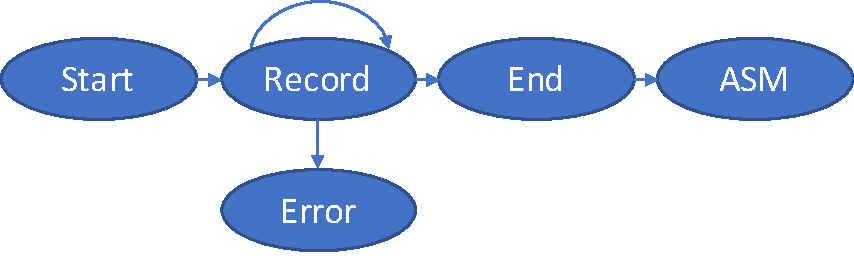
\includegraphics[width=\textwidth]{./Images/FSM.pdf}

\begin{table}[H]
\centering
\caption{States description}
\label{tab:states}
\begin{tabularx}{\textwidth}{|c|X|}
\hline
\multicolumn{1}{|c|}{States}          & \multicolumn{1}{c|}{Description}                     \\\hline
Start                   &
  \begin{tabular}[c]{@{}l@{}}
  Call trace\_start that perform jit\_State setup and \\allocations.
  Change state to LJ\_TRACE\_RECORD.
  \end{tabular}                                                                             \\\hline
Record                  & Recording in progress. It loop over the
	lj\_record\_ins function, which is a huge switch case that record a specific
  bytecode instruction and generate the corresponding specialized IR code of the
  BC before execution. It is executed inside a pcall and jump to the
  \emph{Error} state if a lua exception is thrown. \\\hline%
End                     &
  End of recording. It applies optimizations on the IR (see Chapter \ref{Sec:TO}).        \\\hline
ASM                     &
	Assemble the trace and call trace\_stop to patch the BC (see Chapter \ref{Sec:TA}).     \\\hline
Error                   &
	Abort the recording of the current trace, perform state cleanup, penalize the
	corresponding hot BC or apply blacklisting (see Section \ref{Subsec:abort})                  \\\hline
\end{tabularx}
\end{table}

%===============================================================================
% Abortion and blacklisting
%===============================================================================

\subsection{Abortion and blacklisting}
\label{Subsec:abort}

There exist multiple reason that might cause a recording to abort. Such reason
could be that the unroll limit is reached, that the trace is too long, that the
jit is disabled for a specific function or many others. (see \emph{lj\_traceerr.h}
for the list of possible abort messages). To trigger an abortion, a lua error is
thrown during the recording which transition the recorder state machine to the
\emph{LJ\_TRACE\_ERR} state. Then, the \emph{penalty\_pc} function is called on
the hot bytecode that triggered the recording. The penalty mechanism consists of
a 64-entry table, where each entry is a structure containing the exact PC of the
penalized bytecode, the penalty value, and the reason of the abortion. The
\emph{penaltyslot} variable is a round-robin index inside the table indicating
the next entry to use if a new bytecode needs to be penalized. It as to be noted
that on the contrary of the hotcount mechanism, here the full PC is used to
identify a slot making it free of false positive. However, since the entry is
only 64 entry, penalized bytecode can easily be forgotten in a big code base.
If the penalty for a given bytecode exceeds a threshold then the hot bytecode
responsible for starting the recording gets blacklisted. It means that this
bytecode can never become hot again to start a recording and that if this
bytecode try to be recorded inside another trace, this trace get aborted too
(in most cases). A blacklisted bytecode is never whitelisted by the system.

%===============================================================================
% Intermediate representation
%===============================================================================

\subsection{Intermediate representation}
\label{Subsec:IR}

LuaJIT use a single high-level intermediate representation (IR) across all
optimization stage. As stated, it is generated on the fly during recording and
it is SSA based (static single assignment). It is implemented with a
bidirectional growable array in memory. It includes two different things:
instructions and constants. Instructions are stored at positive indices, while
constants are stored at negative indices. IR references are 16-bits index inside
the IR array and are biased by adding 0x8000 (negative indices are < 0x8000).
All constants are interned and can be compared for equality only by looking at
their references, simplifying many optimization algorithm. Every instruction has
an output data type. Since the Control-flow is flattened, it is always implicit.
Data-flow for loops is represented using PHI-instructions. Other types of
control-flows are managed using guarded instructions. If a guarded instruction
succeeds the normal execution proceed, otherwise the trace is exited. Those
instructions have two purposes, they are generated by the backend to represent
lua branching code and they are used as assertions on operands to test the
validity of assumptions made during recording. If a trace exit is taken the VM
states are restored using the last snapshot. If a trace exit is taken a
sufficient number of times, a child trace is recorded
(trace starting from the exit of a parent trace). Remember that side traces are
not recursive (a side trace cannot have a side trace). The IR is threaded with
segregated, per-opcode skip-list chains. The links are stored in the \emph{prev}
field in the instruction (see Table below). This facilitates low-overhead
lookup for many IR optimizations (i.e. CSE, DSE and alias analysis).

\begin{table}[H]
\centering
\caption{IR instruction format (64 bit)}
\label{tab:ir-format}
\begin{tabular}{|l|c|c|c|c|c|c|}
\hline
\multicolumn{1}{|c|}{size}    & 16              & 16              & 8          & 8          & 8           & 8           \\ \hline
IR after register allocation  & op1             & op2             & t          & o          & r           & s           \\ \hline
IR before register allocation & \multicolumn{2}{c|}{op12/i/gco32} & \multicolumn{2}{c|}{ot} & \multicolumn{2}{c|}{prev} \\ \hline
Constants                     & \multicolumn{6}{c|}{TValue/gco64}                                                       \\ \hline
\end{tabular}
\end{table}

\begin{table}[H]
\centering
\caption{Field definitions.}
\label{tab:ir-field}
\begin{tabular}{|c|l|}
\hline
op1/2 & operands                    \\ \hline
t     & type                        \\ \hline
o     & opcode                      \\ \hline
r     & register allocation         \\ \hline
s     & spill slot                  \\ \hline
prev  & per-opcode skip-list chains \\ \hline
\end{tabular}
\end{table}

%===============================================================================
% Snapshots
%===============================================================================

\subsection{Snapshots}
\label{Subsec:snap}

Snapshot is an important mechanism used in trace compilation. The VM should
always be in a consistent state, meaning that all updates should respect the
original language semantics. However, to perform some trace optimization
(e.g. sinking optimization) this consistency is not respected. Instead
modification that should have occurred during a trace is recorded inside the
snapshots and those modifications are replayed at trace exit. The Snapshot
mechanism is implemented in the snap.[hc] files, and you can find the
\emph{SnapShot} data-structure in lj\_jit.h. For details about
Snapshot usages and implementation refer to section of the wiki on sinking
optimization \cite{luajit-sink} and a mail on the subject \cite{luajit-mail-1}.


    \section{Trace optimizer}
    \label{Sec:TO}
    %!TEX root = ../FYP_Dissertation.tex

We can differentiate in the code, three types of optimizations.
First of all there are the optimizations present in the optimization engine.
They are implemented in the \emph{lj\_opt\_*.c} files and thus easy to spot out.
Those optimization are of two kind, global optimization that are run on the
entire IR at once at the end of the recording phase, during the
\emph{LJ\_TRACE\_END} state (See \ref{Subsec:opt-dce}, \ref{Subsec:opt-loop},
\ref{Subsec:opt-split}, \ref{Subsec:opt-sinking}) and the local optimizations
that are applied while recording a trace (See \ref{Subsec:narrowing},
\ref{Subsubsec:fold}, \ref{Subsubsec:mao}). Finally, there is a plethora of
optimization and heuristic applied here and there (See luaJIT wiki on
optimization \cite{luajit-opt}).

%===============================================================================
% Dead code elimination
%===============================================================================

\subsection{Dead code elimination}
\label{Subsec:opt-dce}

DCE or Dead Code Elimination is performed by the lj\_opt\_dce main function
in two phases. During the first phase called mark snap, it mark all IR
instructions that are referenced by a snapshot. The second phases called
propagate, iteratively mark all IR instruction that are referenced by an already
marked IR instruction while replacing non-marked IR instruction by nops.

%===============================================================================
% Loop optimizations
%===============================================================================

\subsection{Loop optimizations}
\label{Subsec:opt-loop}

The loop optimization is a way to improve code hoisting for trace based around
loops. In fact LuaJIT should try to hoist most invariant instruction and guards
in such a way that trace that doesn't match the current dynamic profile of
the code (assumption on data or type) are exited as soon as possible.
Unfortunately due to the dynamic nature of the IR generated, it contains many
guards a thus, are control-dependent making little room for loop-invariant
code motion (LICM). The solution used here is a copy-substitution of the body
of the loop. It basically consist in always unrolling the loop once before the
actual loop instruction, performing invariant instruction there and making
all the other loop iteration executing only the variant once.

%===============================================================================
% Split optimizations
%===============================================================================

\subsection{Split optimizations}
\label{Subsec:opt-split}

The split optimizations is only use by 32-bits architecture and splits the
64-bits IR instructions into multiple 32-bits onces.

%===============================================================================
% Sinking optimizations
%===============================================================================

\subsection{Sinking optimizations}
\label{Subsec:opt-sinking}
This a very useful optimization that allows to avoid many temporaries and
unnecessary memory accesses and allocations by keeping the values of interest
directly in register. We thus have to remember how the memory should have been
modified in case those access escape our execution path (are not temporary
anymore), for this purpose snapshot are used (See Section \ref{Subsec:snap}).
This optimization is implemented in the \emph{lj\_opt\_sink.c} file. A detailed
explanation of this optimization is available on the wiki \cite{luajit-sink}.

%===============================================================================
% Narrowing optimizations
%===============================================================================

\subsection{Narrowing optimizations}
\label{Subsec:narrowing}

It performs the narrowing of lua numbers (double) into integers when it seems
to be useful. LuaJIT use demand-driven (by the backend) narrowing for index
expressions, integer arguments (FFI), and bit operations and predictive
narrowing for induction variables. It emit overflow check instruction when
necessary. Most arithmetic operations are never narrowed. To learn more on why,
see the comment section in the \emph{lj\_opt\_narrow.c} file.

%===============================================================================
% Fold engine
%===============================================================================

\subsection{Fold engine}
\label{Subsec:fold}

The fold engine implement a rule-based mechanism. Rules are declared using the
LJFOLD macro which contains the IR opcode and a rule on the parametters it
applies to. During the LuaJIT buildvm (more precisely the \emph{buildvm\_fold.c}
file) those rules are scanned and the \emph{lj\_foldef.h} file gets generated.
It contains a semi-perfect hash table for constant-time rule lookup, where each
entry respect the format depicted in Table \ref{tab:fold-format}. It also
contains a second table containing the function to call if a corresponding rule
match.

\begin{table}[H]
\centering
\caption{Fold hash table, bit pattern entry}
\label{tab:fold-format}
\begin{tabular}{|c|c|c|c|c|}
\hline
8                & 7                 & 7                 & 2        & 8                       \\ \hline
index fold table & fold instr opcode & left instr opcode & 00       & right instr opcode      \\ \hline
index fold table & fold instr opcode & left instr opcode & \multicolumn{2}{c|}{literal field} \\ \hline
\end{tabular}
\end{table}

\subsubsection{Fold optimizations}
\label{Subsubsec:fold}

The fold optimizations preformed by the FOLD engine are implemented in the
\emph{lj\_opt\_fold.c} file and can be separated in five well known techniques,
constant folding, algebraic simplifications, reassociation, common subexpression
elimination and Array bounds check elimination.

\subsubsection{Memory access optimizations}
\label{Subsubsec:mao}

The memory access optimization perform by the FOLD engine and implemented
in the lj\_opt\_mem.c file consist of three component, the alias
analysis using high-level semantic disambiguation, Load to load and store to load
forwarding, and finally dead-store elimination.


    \section{Assembler}
    \label{Sec:TA}
    %!TEX root = ../../../FYP_Dissertation.tex

When the recorder state machine reaches the \emph{LJ\_TRACE\_ASM} state, the
\emph{lj\_asm\_trace} main assembler function is called. This function is
responsible for the setup and teardown of the assembler phase. Each IR
instruction of the trace is assembled through the \emph{asm\_ir} function which
is a switch case on the opcode. The implementation of the assembler is divided
in three different files. \emph{lj\_asm.c} contains the assembler code that is
agnostic of the platform, \emph{lj\_asm\_(target).h} contains the assembler code
specific to a particular target (i.e. x86), and \emph{lj\_emit\_(target).h}
contain the helper functions for generating instructions for a specific
instruction-set. A trace is assembled in linear backwards order. It uses
\emph{ASMState} has the main data structure that helps with, physical register
allocation, machine code and IR traversal, and snapshots handling. At the end of
the assembler phase, the bytecode is patched to use instead of the interpreted
bytecode a call to the compiled trace.

% -- TO BE ADDED ????
% in lj_trace.c ? (verify)
% - lj_record_stop
%   - trace stitching (call to c using c API)
%   - end of the hotloop
%   - hit an other already compiled loop (link to it)
%   - return statement
%     - return to interpretor for unhandled cases
%     - when downrec limit reach for side-trace (nagative frame depth)
%     - tail-rec is detected (limit reach in the same framedepth)
%     - limit reach in up recursion (positive frame depth)
%   - hit a compiled function (link to its trace)

  \chapter{Tools}
  \label{Chapt:Tools}

    \section{Verbose mode}
    \label{Sec:Verbose}
    \lhead{Chapter \thechapter. \emph{Verbose mode}}
    %!TEX root = ../FYP_Dissertation.tex

This module shows verbose information about the progress of the
JIT compiler. It prints one line for each generated trace. This module
is useful to see which code has been compiled or where the compiler
punts and falls back to the interpreter.

Example usage:

\begin{lstlisting}
  luajit -jv -e "for i=1,1000 do for j=1,1000 do end end"
  luajit -jv=myapp.out myapp.lua
\end{lstlisting}
To redirect the output to a file, pass a
filename as an argument (use '-' for stdout) or set the environment
variable LUAJIT\_VERBOSEFILE. The file is overwritten every time the
module is started.

The output from the second example could look like this:

\begin{center}
[TRACE   1 myapp.lua:1 loop]

[TRACE   2 (1/3) myapp.lua:1 $->$ 1]
\end{center}

The first number in each line is the internal trace number. Next are
the file name ('myapp.lua') and the line number (':1') where the
trace has started. Side traces also show the parent trace number and
the exit number where they are attached to in parentheses ('(1/3)').
An arrow at the end shows where the trace links to ('$->$ 1'), unless
it loops to itself.

In this case the inner loop gets hot and is traced first, generating
a root trace. Then the last exit from the 1st trace gets hot, too,
and triggers generation of the 2nd trace. The side trace follows the
path along the outer loop and \textit{around} the inner loop, back to its
start, and then links to the 1st trace.

Aborted traces are shown like this:
\begin{center}
[TRACE --- foo.lua:44 -- leaving loop in root trace at foo:lua:50]
\end{center}

Trace aborts are quite common, even in programs which
can be fully compiled. The compiler may retry several times until it
finds a suitable trace. This doesn't work with features that are
not-yet-implemented (NYI error messages). The VM simply falls back to the
interpreter. This may not matter at all if the particular trace is not very high
up in the CPU usage profile, plus the interpreter is quite fast, too.

    \section{Profiler}
    \label{Sec:Profiler}
    \lhead{Chapter \thechapter. \emph{Profiler}}
    %!TEX root = ../FYP_Dissertation.tex

This module is a simple command line interface to the built-in
low-overhead profiler of LuaJIT. The lower-level API of the profiler
is accessible via the "jit.profile" module or the luaJIT\_profile\_* C API.

Example usage:
\begin{lstlisting}
  luajit -jp myapp.lua
  luajit -jp=s myapp.lua
  luajit -jp=-s myapp.lua
  luajit -jp=vl myapp.lua
  luajit -jp=G,profile.txt myapp.lua
\end{lstlisting}
The following dump features are available:
 \begin{itemize}%[label={--}]
  \item \textbf{f} - Shows function name (Default mode).
  \item \textbf{F} - Shows function name with module prepend.
  \item \textbf{l} - Shows line granularity ('module':'line').
  \item \textbf{\textless number\textgreater} - Stack dump depth (callee\textless caller - Default: 1)
  \item \textbf{-\textless number\textgreater} - Inverse stack dump depth (caller\textgreater callee).
  \item \textbf{s} - Split stack dump after first stack level. Implies $\mid depth\mid$
  \textgreater= 2.
  \item \textbf{p} - Show full path for module names.
  \item \textbf{v} - Show VM states (See bellow).
  \item \textbf{z} - Show zones (See bellow).
  \item \textbf{r} - Show raw sample counts (Default: percentages).
  \item \textbf{a} - Annotate excerpts from source code files.
  \item \textbf{A} - Annotate complete source code files.
  \item \textbf{G} - Produce raw output suitable for graphical tools (See bellow).
  \item \textbf{m\textless number\textgreater} - Minimum sample percentage to be shown (Default: 3).
  \item \textbf{i\textless number\textgreater} - Sampling interval in milliseconds (Default: 10).
 \end{itemize}

 Many of those options can be activated at ones.\\

We can also use this module programmatically like in the example bellow. The
\emph{start} function can take 2 arguments, the list of options (describe above)
and the output file.
\begin{lstlisting}[style=LuaStyle]
local prof = require"jit.p"
prof.start("vf", "file.txt")
  -- Code to analyze here
prof.stop()
\end{lstlisting}

\paratitle{VM states:}\\
This options allows to shows the time spent in which state of the VM.
States can be of the following types :

\{Compiled - Interpreted - C code - Garbage Collector - JIT Compiler\} \\

\paratitle{Zone:}\\
statistics can be grouped in user defined zone. Bellow is an example a such a
definition.
\begin{lstlisting}
    local zone = require("jit.zone")
    zone("MyZone")
      -- Lua code here
    zone()
\end{lstlisting}

\paratitle{Graphical tools:}\\
This option can be used to graphically show the dump in a nice image format
(see Appendix \ref{Apendix:fl})

    \section{Dump mode}
    \label{Sec:Dump-mode}
    \lhead{Chapter \thechapter. \emph{Dump mode}}
    %!TEX root = ../../../FYP_Dissertation.tex

%===============================================================================
% How to use it
%===============================================================================

\subsection{How to use it}
\label{Subsec:dump-usage}

This module can be used to debug the JIT compiler itself or to analyze its
behavior regarding a piece of code. It dumps the
code representations and structures used in various compiler stages.

Example usage:
\begin{lstlisting}
  luajit -jdump -e "
    local x=0
    for i=1,1e6 do x=x+i end
    print(x)
  "
  luajit -jdump=im -e "
    for i=1,1000 do
      for j=1,1000 do end
    end
  " | less -R
  luajit -jdump=is myapp.lua | less -R
  luajit -jdump=-b myapp.lua
  luajit -jdump=+aH,myapp.html myapp.lua
  luajit -jdump=ixT,myapp.dump myapp.lua
\end{lstlisting}
The first argument specifies the dump mode. The second argument gives
the output file name. Default output is to stdout, unless the environment
variable LUAJIT\_DUMPFILE is set. The file is overwritten every time the
module is started. Different features can be turned on or off with the dump mode.
If the mode starts with a '+', the following features are added to the default
set of features; a '-' removes them. Otherwise the features are replaced.\\
The following dump features are available (* marks the default):

\begin{itemize}
  \item \textbf{t *} - Print a line for each started, ended or aborted trace (see also -jv).
  \item \textbf{b *} - Dump the traced bytecode.
  \item \textbf{i *} - Dump the IR (intermediate representation).
  \item \textbf{r} - Augment the IR with register/stack slots.
  \item \textbf{s} - Dump the snapshot map.
  \item \textbf{m *} - Dump the generated machine code.
  \item \textbf{x} - Print each taken trace exit.
  \item \textbf{X} - Print each taken trace exit and the contents of all registers.
  \item \textbf{a} - Print the IR of aborted traces, too.
\end{itemize}
The output format can be set with the following characters:
\begin{itemize}
   \item \textbf{T} - Plain text output.
   \item \textbf{A} - ANSI-colored text output
   \item \textbf{H} - Colorized HTML + CSS output.
\end{itemize}
The default output format is plain text. It's set to ANSI-colored text
if the COLORTERM variable is set.

We can also use this module programmatically like in the example below. The
\emph{on} function can take 2 arguments, the list of options (describe above)
and the output file.
\begin{lstlisting}[style=LuaStyle]
local dump = require"jit.dump"
dump.on("tbimT", "outfile.txt")
  -- Code to analyze here
dump.off()
\end{lstlisting}

%===============================================================================
% Understanding states dump
%===============================================================================

\subsection{Understanding states dump}
\label{Subsec:dump-states}

This command looks like the verbose mode (-jv) and print information for each start,
end or abortion of a trace. The output can have one of those three shapes.
\begin{verbatim}
---- TRACE 1 start foo.lua:125
---- TRACE 1 stop -> [link]
---- TRACE 1 abort foo.lua:142 -- [message]
\end{verbatim}
The first one is emitted when a recording starts. It shows the potential
trace number, the file and the source line where that trace start.
The second one is emitted when a trace has been successfully recorded. In
addition to the trace number, it shows to what the trace link to (See Table
\ref{tab:dump-link} for [link] possible values). Finally, the last one is emitted
when the recording of a trace is aborted. It shows the file and the source line
responsible for the abortion and print a [message] depicting the reason. For
a list of possible messages see TraceError in lj\_trace.h and macro in
lj\_traceerr.h.

\paratitle{Side trace}\\
When instruction of a trace marked as guard fail, the normal execution of a
trace is interrupted. We then call that spot a side exit of the trace. When a
given side exit is taken enough time, it is said to be hot and generate a new
trace starting from it. This new trace is called a side trace of the first one
called the parent trace. Below is how the start of the recording of a side
trace is shown in the dump.
\begin{verbatim}
---- TRACE 30 start 21/0 foo.lua:103
\end{verbatim}
Here 30 is the side trace number, 21 the parent trace from which the side trace
start from and 0 is the side exit number.

\paratitle{Stitching}\\
Trace stitching is a feature which allows traces to stop at a classic C function
or a not-compiled built-in, return to the interpreter, run the C function or
built-in and then start a new trace after it returns. Below is an example of
how trace stitching due to a not-compiled built-in can be shown in the dump.
\begin{verbatim}
---- TRACE 1 start foo.lua:6
  [...]
  0000  . FUNCC               ; os.clock
---- TRACE 1 stop -> stitch
---- TRACE 2 start 1/stitch foo.lua:35
\end{verbatim}
As you can see the trace prior to the stitching has its link marked as
\emph{stitch} and the one after is shown like a side trace but with
\emph{stitch} instead of the number of the side exit.

%===============================================================================
% Understanding BC dump
%===============================================================================

\subsection{Understanding BC dump}
\label{Subsec:dump-bc}

Below is an example of how a BC instruction is shown in the dump. For a complete
list of BC instruction and their corresponding arguments look at the wiki page
\cite{luajit-bc}.
\begin{verbatim}
0007  . . CALL     2   2   2  ;comment
\end{verbatim}
\begin{itemize}
  \item 1st column : bc number, numbered by function.
  \item 2nd column : The dots represent the depth (call hierarchy).
  \item 3rd column : bc instruction.
  \item other-1... : bc arguments.
  \item last       : comment helping to tie the instruction to the lua code.
\end{itemize}

%===============================================================================
% Understanding IR dump
%===============================================================================

\subsection{Understanding IR dump}
\label{Subsec:dump-ir}

Below are some example of dumps of IR instructions.
\begin{verbatim}
0001 rax   >  tab SLOAD  #46   T
0014 rbp      int TOBIT  0005  bias
0040 [1c]  >  tab HLOAD  0039
0035  {sink}+ cdt CNEW   +16
0023  {0021}  num XSTORE 0022  0018
0155       >  p32 HREFK  0154  "assert" @131
0159       >  fun EQ     0158  madl_gutil.mad:298
\end{verbatim}

\begin{itemize}
  \item 1st column: IR instruction number (numbered per trace)
  \item 2nd column: Show where the value is written to when converted to machine
    code. This column is only present if the 'r' flags is included in -jdump,
    which augments the IR with register/stack slots. It is not part of the IR
    itself.
    \begin{itemize}
      \item '\%w' : physical CPU register
      \item '[\%d+]' : physical CPU stack slot (hexadecimal offset from stack pointer).
      \item \{sink\} : Show when a \emph{sink} optimization occur.
      \item \{\%d+\} : Refers to the IR instruction where a \emph{sink}
        optimization occur.
    \end{itemize}
  \item 3nd column: Instruction flags (See lj\_ir.h)
  \begin{itemize}
    \item "\textgreater" (IRT\_GUARD) are locations of
        guards (leading to possible side exits from the trace).
    \item "+" (IRT\_ISPHI) indicates
        instruction is left or right PHI operand. (i.e referred
        to in some PHI instruction).
  \end{itemize}
  \item 4rd column: IR type.
  \item 5th column: IR opcode.
  \item 6th/7th column: IR operands
    \begin{itemize}
      \item '\%d+' : reference to IR instruction (SSA ref).
      \item '\#' : prefixes refer to slot numbers, used in SLOADS.
        \#0 is the base frame (modified only in tail calls).
        \#1 is the first slot in the first frame (register 0 in
        the bytecode).
      \item '(+$\vert$-)\%d+' : prefixes indicate positive or negative numeric literals.
      \item '[0x\%d+]$\vert$NULL' : memory addresses.
      \item '"..."' : strings.
      \item '@\%d+' : indicate slot where the value of a key is to be found (in a table).
      \item 'bias' : Used by \emph{TOBIT} represent the constant
        $2^{52}+2^{51}$ added to the FP number.
      \item \{0x\%d+\} : lua table.
      \item 'userdata:\%p' : user data.
      \item 'my\_func:ligne' : functions.
      \item '(...)' : function arguments for call-type IR.
    \end{itemize}
    To see possible argument values for some specific instruction see Table
    \ref{tab:dump-sload} to \ref{tab:dump-tostr}.
\end{itemize}


\paratitle{Snapshot}\\
Each snapshot (SNAP), lists the modified stack slots and the corresponding values.
Below are two examples of how snapshots are shown in IR dump. For further
comments on why snapshots are used, see Section \ref{Subsec:snap}. Below is an
example of how snapshot can be shown in the dump.
\begin{verbatim}
....    SNAP   #1   [ ---- ---- ---- ---- 0069 0070 0071 ---- ]
....    SNAP   #1   [ foo.lua:120|---- ---- false ]
\end{verbatim}
The i-th value in the snapshot list represents the IR instruction number of the
instruction that wrote a value in slot number i. '- - - -' indicates that the slot
has not been modified. Function frames are separated by '$\vert$'.

%===============================================================================
% Understanding mcode dump
%===============================================================================

\subsection{Understanding mcode dump}
\label{Subsec:dump-mcode}

Below is an example of a small typical trace. It starts with some initialization
followed most of the time by a loop part clearly indicated by the label.
Each line is composed of two parts, the mcode instruction's address and the
corresponding assembler instruction.
\begin{verbatim}
10020ff93  mov dword [0x00041410], 0x1
10020ff9e  cvttsd2si ebp, [rdx+0x10]
10020ffa3  xorps xmm7, xmm7
10020ffa6  cvtsi2sd xmm7, ebp
10020ffaa  cmp ebp, +0x5a
10020ffad  jz 0x100200014 ->1
10020ffb3  cmp dword [rdx+0x4], 0xfffeffff
10020ffba  jnb 0x100200018  ->2
10020ffc0  addsd xmm7, [rdx]
10020ffc4  add ebp, +0x01
10020ffc7  cmp ebp, +0x64
10020ffca  jg 0x10020001c ->3
->LOOP:
10020ffd0  xorps xmm6, xmm6
10020ffd3  cvtsi2sd xmm6, ebp
10020ffd7  cmp ebp, +0x5a
10020ffda  jz 0x100200024 ->5
10020ffe0  addsd xmm7, xmm6
10020ffe4  add ebp, +0x01
10020ffe7  cmp ebp, +0x64
10020ffea  jle 0x10020ffd0  ->LOOP
10020ffec  jmp 0x100200028  ->6
\end{verbatim}

%===============================================================================
% How does it works
%===============================================================================

\subsection{How does it works}
\label{Subsec:dump-internals}

This section briefly presents the parts of the code of luaJIT involved in the process of
emitting the dump. The dump module (dump.lua) is responsible for the set up of the
jit to emit traces and also for printing the results in a human understandable
format. Depending on the dump it has to print (with respect to the provided
parameters, see Section \ref{Subsec:dump-usage}) it attaches some handler
(callback lua function) to specific VM events using jit\_attach (see lib\_jit.c).
The predefined VM event used here are : BC, TRACE, RECORD, TEXIT
(see VMEvent in lj\_vmevent.h). In the jit, lj\_vmevent\_send (see lj\_vmevent.h)
is used to send a VM event, lj\_vmevent\_prepare to find the handler attached to a
specific event and lj\_vmevent\_call to call it (see lj\_vmevent.c).
The lua module uses more function from lib\_jit.c (all jutil.* function
in dump.lua) to extract more information.


    \section{Valgrind}
    \label{Sec:Valgrind}
    \lhead{Chapter \thechapter. \emph{Valgrind}}
    %!TEX root = ../FYP_Dissertation.tex

Valgrind is an instrumentation framework for building dynamic analysis tools.
There are Valgrind tools that can automatically detect many memory management
and threading bugs, and profile programs in detail (cf \cite{valgrind}). To be
able to debug your c code used through ffi with Valgrind, LuaJIT needs to be
compiled with specific options. Some information on that, can be found in the
LuaJIT \emph{Makefile} but a summary of the way to proceed for linux is describe
here. First we need to uncomment in \emph{src/makefile}, \emph{CCDEBUG} to
allow for debug information, \emph{DLUAJIT\_USE\_SYSMALLOC} to use the system
allocator (to get useful memcheck information), \emph{DLUAJIT\_USE\_VALGRIND}
and \emph{DLUAJIT\_ENABLE\_GC64} if run on a x64 platform. After recompiling
with those options, you will need the suppression file \emph{src/lj.supp}
(containing known false positive for memcheck) to run a valgrind command such as
the following.

\begin{lstlisting}[style=CStyle]
valgrind
		--tool=memcheck
		--leak-check=full
		--track-origins=yes
		--log-file='log.txt'
		--suppressions=lj.supp
		./luajit myprogram
\end{lstlisting}




%--------------------------------------------------------------------------------
% Prints out any appendices (comment/delete if you do not need any)
%--------------------------------------------------------------------------------
\clearpage
\addtocontents{toc}{\vspace{2em}}
\appendix
\baselineskip=16pt

% \chapter{Files hierarchy}
% \label{Apendix:files}
% \lhead{Appendix \ref{Apendix:files}. \emph{Files hierarchy}}
% %!TEX root = ../FYP_Dissertation.tex
\paratitle{dynasm/*:}\\
All files in this folder correspond to the Dynamic Assembler (see Apendix \ref{Apendix:DynASM})\\
\paratitle{dynasm/dasm\_*.h:}\\
DynASM encoding engine for a specific architecture.\\
\paratitle{dynasm/dasm\_*.lua:}\\{}
DynASM lua module for a specific architecture.\\
\paratitle{dynasm/dynasm.lua:}\\
DynASM mechanism main source file.\\
\paratitle{src/host/*:}\\
The files in this directory are only used during the build process of LuaJIT.
For cross-compilation, they must be executed on the host, not on the target.\\
\paratitle{src/host/buildvm.c:}\\
\paratitle{src/host/buildvm.h:}\\
\paratitle{src/host/buildvm\_asm.c:}\\
\paratitle{src/host/buildvm\_fold.c:}\\
\paratitle{src/host/buildvm\_lib.c:}\\
\paratitle{src/host/buildvm\_libbc.h:}\\
\paratitle{src/host/buildvm\_peobj.c:}\\
\paratitle{src/host/genlibbc.lua:}\\
\paratitle{src/host/genminilua.lua:}\\
\paratitle{src/host/minilua.c:}\\
Minimal copy of Lua 5.1 used to build LuaJIT.\\
\paratitle{src/jit/bc.lua:}\\
\paratitle{src/jit/bcsave.lua:}\\
Lua module used to save the bc of a source file.\\
\paratitle{src/jit/dis\_*.lua:}\\
LuaJIT disassembler module for a specific architecture, used as a help module by
the dumper mode to dump code of generated trace (See dump.lua).\\
\paratitle{src/jit/dump.lua:}\\
LuaJIT compiler dump module (see Chapter \ref{Chapt:Dump-mode}).\\
\paratitle{src/jit/p.lua:}\\
LuaJIT profiler (see Chapter \ref{Chapt:Profiler}).\\
\paratitle{src/jit/v.lua:}\\
LuaJIT verbose mode (see Chapter \ref{Chapt:Verbose}).\\
\paratitle{src/jit/zone.lua:}\\
This module implements a simple hierarchical zone model
(See \emph{zone} in Chapter \ref{Chapt:Profiler}).\\
\paratitle{src/lauxlib.h:}\\
Auxiliary library for the Lua/C API.\\
\paratitle{src/lib\_*.c:}\\
Implement a library with an interface available through lua code.\\
\paratitle{src/lib\_aux.c:}\\
\paratitle{src/lib\_aux.c:}\\
\paratitle{src/lib\_base.c:}\\
\paratitle{src/lib\_bit.c:}\\
\paratitle{src/lib\_debug.c:}\\
\paratitle{src/lib\_ffi.c:}\\
FFI library.\\
\paratitle{src/lib\_init.c:}\\
\paratitle{src/lib\_io.c:}\\
\paratitle{src/lib\_jit.c:}\\
\paratitle{src/lib\_math.c:}\\
\paratitle{src/lib\_os.c:}\\
\paratitle{src/lib\_package.c:}\\
\paratitle{src/lib\_string.c:}\\
\paratitle{src/lib\_table.c:}\\
\paratitle{src/lj\_alloc.[ch]:}\\
Bundled memory allocator.\\
\paratitle{src/lj\_api.c:}\\
Lua/c api (e.g. stack handling)\\
\paratitle{src/lj\_arch.h:}\\
\paratitle{src/lj\_asm.[ch]:}\\
Generic code for assembling a trace.\\
\paratitle{src/lj\_asm\_*.h:}\\
IR assembler, convert SSA IR into machine code for a specific architecture.\\
\paratitle{src/lj\_bc.[ch]:}\\
Bytecode instruction format.\\
\paratitle{src/lj\_bcdump.h:}\\
\paratitle{src/lj\_bcread.c:}\\
Bytecode reader to allow executing saved bc.\\
\paratitle{src/lj\_bcwrite.c:}\\
Bytecode writer to save bc.\\
\paratitle{src/lj\_buf.c:}\\
\paratitle{src/lj\_buf.h:}\\
\paratitle{src/lj\_carith.[ch]:}\\
C data arithmetic.\\
\paratitle{src/lj\_ccall.[ch]:}\\
FFI C call handling.\\
\paratitle{src/lj\_ccallback.[ch]:}\\
FFI C callback handling.\\
\paratitle{src/lj\_cconv.[ch]:}\\
C type conversions.\\
\paratitle{src/lj\_cdata.[ch]:}\\
C data management.\\
\paratitle{src/lj\_char.c:}\\
\paratitle{src/lj\_char.h:}\\
\paratitle{src/lj\_clib.[ch]:}\\
FFI C library loader.\\
\paratitle{src/lj\_cparse.[ch]:}\\
C declaration parser.\\
\paratitle{src/lj\_crecord.c:}\\
\paratitle{src/lj\_crecord.h:}\\
\paratitle{src/lj\_ctype.[ch]:}\\
C type management.\\
\paratitle{src/lj\_debug.c:}\\
\paratitle{src/lj\_debug.h:}\\
\paratitle{src/lj\_def.h:}\\
\paratitle{src/lj\_dispatch.c:}\\
\paratitle{src/lj\_dispatch.h:}\\
\paratitle{src/lj\_emit\_*.h:}\\
Instruction emitter for a specific architecture.\\
\paratitle{src/lj\_err.c:}\\
\paratitle{src/lj\_err.h:}\\
\paratitle{src/lj\_errmsg.h:}\\
\paratitle{src/lj\_ff.h:}\\
\paratitle{src/lj\_ffrecord.c:}\\
\paratitle{src/lj\_ffrecord.h:}\\
\paratitle{src/lj\_frame.h:}\\
\paratitle{src/lj\_func.[ch]:}\\
Function handling, prototype and upvalues.\\
\paratitle{src/lj\_gc.[ch]:}\\
Garbage collector implementation\\
\paratitle{src/lj\_gdbjit.c:}\\
\paratitle{src/lj\_gdbjit.h:}\\
\paratitle{src/lj\_ir.c:}\\
\paratitle{src/lj\_ir.h:}\\
\paratitle{src/lj\_ircall.h:}\\
\paratitle{src/lj\_jit.h:}\\
\paratitle{src/lj\_lex.c:}\\
Lexer (Lexical analyzer) for lua code.\\
\paratitle{src/lj\_lex.h:}\\
Main header file used during the lexer, parser and bcreader.\\
\paratitle{src/lj\_lib.c:}\\
\paratitle{src/lj\_lib.h:}\\
\paratitle{src/lj\_load.c:}\\
\paratitle{src/lj\_mcode.c:}\\
\paratitle{src/lj\_mcode.h:}\\
\paratitle{src/lj\_meta.c:}\\
\paratitle{src/lj\_meta.h:}\\
\paratitle{src/lj\_obj.c:}\\
\paratitle{src/lj\_obj.h:}\\
\paratitle{src/lj\_iropt.h:}\\
Common header for IR emitter and optimizations.\\
\paratitle{src/lj\_opt\_*.c:}\\
IR optimization implementation for a specific type of optimization.\\
\paratitle{src/lj\_parse.[ch]:}\\
Lua parser and bc generator\\
\paratitle{src/lj\_profile.c:}\\
\paratitle{src/lj\_profile.h:}\\
\paratitle{src/lj\_record.[ch]:}\\
Trace recorder converts bytecode into SSA IR.\\
\paratitle{src/lj\_snap.[ch]:}\\
Creates and handles trace snapshots.\\
\paratitle{src/lj\_state.c:}\\
\paratitle{src/lj\_state.h:}\\
\paratitle{src/lj\_str.[ch]:}\\
Internal String handling.\\
\paratitle{src/lj\_strfmt.c:}\\
\paratitle{src/lj\_strfmt.h:}\\
\paratitle{src/lj\_strfmt\_num.c:}\\
\paratitle{src/lj\_strscan.c:}\\
\paratitle{src/lj\_strscan.h:}\\
\paratitle{src/lj\_tab.[ch]:}\\
Lua table handling.
\paratitle{src/lj\_target.h:}\\
Generic definitions for target CPU.\\
\paratitle{src/lj\_target\_*.h:}\\
Definitions for target CPU for a specific architecture.\\
\paratitle{src/lj\_trace.[ch]:}\\
Trace management.\\
\paratitle{src/lj\_traceerr.h:}\\
\paratitle{src/lj\_udata.c:}\\
\paratitle{src/lj\_udata.h:}\\
\paratitle{src/lj\_vm.h:}\\
\paratitle{src/lj\_vmevent.c:}\\
\paratitle{src/lj\_vmevent.h:}\\
\paratitle{src/lj\_vmmath.c:}\\
\paratitle{src/ljamalg.c:}\\
LuaJIT core and libraries amalgamation (Used in amalg compilation target to generate better binaries).\\
\paratitle{src/lua.h:}\\
\paratitle{src/lua.hpp:}\\
\paratitle{src/luaconf.h:}\\
\paratitle{src/luajit.c:}\\
\paratitle{src/luajit.h:}\\
\paratitle{src/lualib.h:}\\
\paratitle{src/msvcbuild.bat:}\\
\paratitle{src/ps4build.bat:}\\
\paratitle{src/psvitabuild.bat:}\\
\paratitle{src/vm\_*.dasc:}\\
Virtual Machine written using DynASM for a specific architecture (see Chapter \ref{Chapt:DynASM} for DynASM and Part \ref{Part:VM} for the VM)\\
\paratitle{src/xb1build.bat:}\\
\paratitle{src/xedkbuild.bat:}\\

% \chapter{Data structure}
% \label{Apendix:ds}
% \lhead{Appendix \ref{Apendix:ds}. \emph{Data structure}}

\chapter{Dump values}
\label{Apendix:dump-values}
\lhead{Appendix \ref{Apendix:dump-values}. \emph{Dump values}}
%!TEX root = ../FYP_Dissertation.tex

In this appendix, is presented possible values that can be shown in some dump
and their corresponding meaning.
\begin{table}
\centering
\begin{tabular}{|l|l|}
\hline
\multicolumn{1}{|c|}{value} & \multicolumn{1}{c|}{Meaning}\\\hline
none                        & Incomplete trace. No link, yet.\\
root                        & Link to other root trace.\\
loop                        & Loop to same trace.\\
tail-recursion              & Tail-recursion.\\
up-recursion                & Up-recursion.\\
down-recursion              & Down-recursion.\\\hline
\multirow{2}{*}{interpreter}& Fallback to interpreter (stop a side trace record due\\
& to maximum reached see \emph{sidecheck:} in lj\_record.c)\\\hline
return                      & Return to interpreter.\\
stitch                      & race stitching.\\\hline
\end{tabular}
\caption{
  Possible value for [link] \\(See jit\_trlinkname and TraceLink in lib\_jit.c
  and lj\_jit.h)
}
\label{tab:dump-link}
\end{table}
\begin{table}
\centering
\begin{tabular}{|l|l|l|}
\hline
P & IRSLOAD\_PARENT    & Coalesce with parent trace.\\
F & IRSLOAD\_FRAME     & Load 32 bits of ftsz.\\
T & IRSLOAD\_TYPECHECK & Needs type check.\\
C & IRSLOAD\_CONVERT   & Number to integer conversion.\\
R & IRSLOAD\_READONLY  & Read-only, omit slot store.\\
I & IRSLOAD\_INHERIT   & Inherited by exits/side traces.\\
\hline
\end{tabular}
\caption{
  Possible value for SLOAD argument \\(See lj\_ir.h)
}
\label{tab:dump-sload}
\end{table}
\begin{table}
\centering
\begin{tabular}{|l|l|l|}
\hline
R & IRXLOAD\_READONLY  & Load from read-only data.\\
V & IRXLOAD\_VOLATILE  & Load from volatile data.\\
U & IRXLOAD\_UNALIGNED & Unaligned load.\\
\hline
\end{tabular}
\caption{
  Possible value for XLOAD argument \\(See lj\_ir.h)
}
\label{tab:dump-xload}
\end{table}
\begin{table}
\centering
\begin{tabular}{|l|l|l|}
\hline
str.len        & IRFL\_STR\_LEN        & \\
func.env       & IRFL\_FUNC\_ENV       & \\
func.pc        & IRFL\_FUNC\_PC        & \\
func.ffid      & IRFL\_FUNC\_FFID      & Function id\\
thread.env     & IRFL\_THREAD\_ENV     & \\
tab.meta       & IRFL\_TAB\_META       & \\
tab.array      & IRFL\_TAB\_ARRAY      & \\
tab.node       & IRFL\_TAB\_NODE       & Hash part\\
tab.asize      & IRFL\_TAB\_ASIZE      & Size of array part\\
tab.hmask      & IRFL\_TAB\_HMASK      & Size of hash part - 1\\\hline
\multirow{3}{*}{tab.nomm} & \multirow{3}{*}{IRFL\_TAB\_NOMM} & Negative cache for fast \\
& & metamethods bitmap, marking\\
& & absent fields of the metatable\\\hline
udata.meta     & IRFL\_UDATA\_META     & \\
udata.udtype   & IRFL\_UDATA\_UDTYPE   & See UDTYPE table\\
udata.file     & IRFL\_UDATA\_FILE     & udata payload \\
cdata.ctypeid  & IRFL\_CDATA\_CTYPEID  & \\
cdata.ptr      & IRFL\_CDATA\_PTR      & cdata payload \\
cdata.int      & IRFL\_CDATA\_INT      & cdata payload \\
cdata.int64    & IRFL\_CDATA\_INT64    & cdata payload \\
cdata.int64\_4 & IRFL\_CDATA\_INT64\_4 & cdata payload \\
\hline
\end{tabular}
\caption{
  Possible value for FLOAD or FREF argument \\(See lj\_ir.h)
}
\label{tab:dump-fload-fref}
\end{table}
\begin{table}
\centering
\begin{tabular}{|l|l|}
\hline
UDTYPE\_USERDATA  & Regular userdata.\\
UDTYPE\_IO\_FILE  & I/O library FILE.\\
UDTYPE\_FFI\_CLIB & FFI C library namespace.\\\hline
\end{tabular}
\caption{
  Possible value for userdata types \\(See lj\_obj.h)
}
\label{tab:dump-udata}
\end{table}
\begin{table}
\centering
\begin{tabular}{|l|l|}
\hline
floor & FPM\_FLOOR \\
ceil  & FPM\_CEIL  \\
trunc & FPM\_TRUNC \\
sqrt  & FPM\_SQRT  \\
exp   & FPM\_EXP   \\
exp2  & FPM\_EXP2  \\
log   & FPM\_LOG   \\
log2  & FPM\_LOG2  \\
log10 & FPM\_LOG10 \\
sin   & FPM\_SIN   \\
cos   & FPM\_COS   \\
tan   & FPM\_TAN   \\
\hline
\end{tabular}
\caption{
  Possible value for FPMATH argument \\(See lj\_ir.h)
}
\label{tab:dump-fpmath}
\end{table}
\begin{table}
\centering
\begin{tabular}{|l|l|}
\hline
IRBUFHDR\_RESET  & Reset buffer \\
IRBUFHDR\_APPEND & Append to buffer \\
\hline
\end{tabular}
\caption{
  Possible value for BUFHDR argument \\(See lj\_ir.h)
}
\label{tab:dump-bufhdr}
\end{table}

\begin{table}
\centering
\begin{tabular}{|l|l|l|}
\hline
INT  & IRTOSTR\_INT  & Convert integer to string.  \\
NUM  & IRTOSTR\_NUM  & Convert number to string.  \\
CHAR & IRTOSTR\_CHAR & Convert char value to string.  \\\hline
\end{tabular}
\caption{
  Possible value for TOSTR argument \\(See lj\_ir.h)
}
\label{tab:dump-tostr}
\end{table}

\chapter{Flame graphs}
\label{Apendix:fl}
\lhead{Appendix \ref{Apendix:fl}. \emph{Flame graphs}}
%!TEX root = ../FYP_Dissertation.tex
First we need to get the FlameGraph \cite{flamegraph} tool.
\begin{center}
\begin{lstlisting}
  git clone https://github.com/brendangregg/FlameGraph
\end{lstlisting}
\end{center}
Then we need to, generate the raw dump from luajit and use FlameGraph to generate
the svg file. Assuming \emph{\$flamegraph} contains the path to the tool (/FlameGraph/flamegraph.pl)

\begin{center}
\begin{lstlisting}
  export flamegraph=./FlameGraph/flamegraph.pl
  luajit -jp=G,myapp.out myapp.lua
  $flamegraph myapp.out > myapp.svg
\end{lstlisting}
\end{center}
Then you can open myapp.svg with your favorite viewer.


\chapter{DynASM: Assembler}
\label{Apendix:DynASM}
\lhead{Appendix \ref{Apendix:DynASM}. \emph{DynASM: Assembler}}
%!TEX root = ../../FYP_Dissertation.tex

DynASM is a Dynamic Assembler for code generation engines, it has been developed
primarily as a tool for LuaJIT and its source code can be found in the dynasm
folder of the LuaJIT project \cite{luajit-src}. It is currently used in LuaJIT
v2 has a tool to write the fast VM interpreting the bytecode. It supports the
following platforms : x86, x64, ARM, PowerPC, and MIPS. An unofficial
documentation with tutorials is available \cite{dynasm}. In the remaining part
of this appendix, a minimum amount of information is presented to give the
ability to read and understand a DynASM file (\emph{.dasc}).


\paratitle{Main directives}

\begin{itemize}
    \item \keyword{.arch} : Specifies the architecture of the assembly code.
    \item \keyword{.type} name, ctype [, default\_reg] : Makes easier to manipulate registers of type \emph{ctype*}. The provided syntactic sugar is depicted in
Table~\ref{tab:type-sugar}.
    \item \keyword{.macro} [...] \keyword{.endmacro} : Create a multi-lines
macro instruction that can be invoked as a normal instruction and where arguments
will be substituted.
    \item \keyword{.define} : Defines a prepreprocessor substitution.
    \item \keyword{.if} [...] \keyword{.elif} [...] \keyword{.else} [...] \keyword{.endif} : Preprocessor conditional construct similar as c preprocessor.
\end{itemize}

\begin{table}
\centering
\begin{tabular}{|l|l|}
\hline
\multicolumn{1}{|c|}{Sugar} & \multicolumn{1}{c|}{Expansion} \\\hline
\#name                      & sizeof(ctype)\\
name:reg-\textgreater field & [reg + offsetof(ctype,field)]\\
name:reg[imm32]             & [reg + sizeof(ctype)*imm32]\\
name:reg[imm32].field       & [reg + sizeof(ctype)*imm32 + offsetof(ctype,field)]\\
name:reg...                 & [reg + (int)(ptrdiff\_t)\&(((ctype*)0)...)]\\\hline
\end{tabular}
\caption{Syntactic sugar provided by \keyword{.type} macro}
\label{tab:type-sugar}
\end{table}

\paratitle{Line markers}\\
Typical DynASM lines that emit some assembler instructions has to start with a
vertical bare ("$\vert$"). If we want to emit some lines of \emph{C} code but
still want DynASM's preprocessor to do substitutions, they must start with a double vertical bar ("$\vert\vert$"). Finally lines with no starting markers are
truly untouched and discarded by DynASM. To be noted that lines of \emph{C} code that
has to be inlined with a macro must start with a double vertical bar. \\

\paratitle{Labels}\\
They exist multiple types of labels to refer to. The first category is global
labels that have two types, static label ($\vert-$\textgreater name:) and dynamic ones ($\vert$=\textgreater imm32:).
Those labels have to be unique in a DynASM file. The second category is local
labels that use a single digit from 1 to 9 ($\vert$i:). They can be defined
multiple times inside a same DynASM file and are used by jump instructions by
means of the syntax \textless i or \textgreater i. They respectively point to
the most recent, the next definition of i as the jump target.


\addtocontents{toc}{\vspace{2em}} % Add a gap in the Contents, for aesthetics

\backmatter

%--------------------------------------------------------------------------------
% Prints out the bibliography
%--------------------------------------------------------------------------------

\label{Bibliography}

\lhead{\emph{Bibliography}}
\renewcommand{\bibname}{References}
\bibliographystyle{MyBibliographyStyle}
\bibliography{./Tex/FYPBibliography}


\end{document}